 %=====================================================================
%  MANUSCRIPT PREPARATION & AUTHOR NOTES
%  Title: Spatiotemporal Trajectory Engineering in Bioactive Silicate Ceramics
%  Target Journal: Journal of Functional Biomaterials (MDPI)
%  Article Type: Original Research Article
%=====================================================================
%  SUBMISSION & COMPILATION CHECKLIST:
%   - Engine: Compile with pdflatex (all figures TikZ-native, vector output).
%   - Cross-references: Run pdflatex twice to resolve all equations, figures, and tables.
%   - Citation Style: Sequential numerical format [1], [2], [3] matching MDPI guidelines.
%   - Metadata: DOIs verified against primary publisher metadata.
%=====================================================================
\documentclass[11pt]{article}


% ================= PACKAGES =================
\usepackage[a4paper, margin=2.0cm, headheight=14pt, headsep=12pt]{geometry}
\usepackage{times}
\usepackage[utf8]{inputenc}
\usepackage[T1]{fontenc}
\usepackage{amsmath,amssymb}
\usepackage{graphicx}
\usepackage{booktabs}
\usepackage{longtable}
\usepackage{array}
\usepackage{xcolor}
\usepackage{colortbl}
\usepackage{titlesec}
\usepackage{enumitem}
\usepackage{hyperref}
\usepackage{caption}
\usepackage{multirow}
\usepackage{fancyhdr}
\usepackage{setspace}
\usepackage{multicol}
\usepackage{tikz}
\usetikzlibrary{arrows.meta,positioning,shapes.geometric,fit,backgrounds,calc,patterns}
\usepackage{float}
\usepackage[version=4]{mhchem}
\usepackage{siunitx}
\usepackage{subcaption}
\usepackage{microtype}


% ---- Spacing ----
\onehalfspacing
\setlength{\parskip}{3pt}
\setlength{\parindent}{12pt}


% ---- Table typography ----
\newcommand{\tablesize}{\fontsize{8.5pt}{10pt}\selectfont}
\renewcommand{\arraystretch}{1.12}
\setlength{\tabcolsep}{4pt}


% ---- Caption setup ----
\captionsetup{font=small,skip=6pt}
\setlength{\abovecaptionskip}{8pt}
\setlength{\belowcaptionskip}{6pt}


% ---- Color palette ----
\definecolor{chemblue}{RGB}{29,78,137}
\definecolor{archgreen}{RGB}{15,118,110}
\definecolor{statepurple}{RGB}{88,44,131}
\definecolor{bioamber}{RGB}{180,83,9}
\definecolor{rtzred}{RGB}{153,27,27}
\definecolor{coregray}{RGB}{85,85,95}
\definecolor{gelcyan}{RGB}{0,125,135}
\definecolor{arrowgray}{RGB}{55,65,81}
\definecolor{ukblue}{RGB}{222,235,247}
\definecolor{ukgreen}{RGB}{232,248,244}
\definecolor{ukpurple}{RGB}{243,236,249}
\definecolor{ukamber}{RGB}{252,242,221}
\definecolor{ukred}{RGB}{253,227,226}


% ---- Column types ----
\newcolumntype{L}[1]{>{\raggedright\arraybackslash}p{#1}}
\newcolumntype{C}[1]{>{\centering\arraybackslash}p{#1}}


% ---- Hyperref ----
\hypersetup{
    colorlinks=true,
    linkcolor=blue!65!black,
    citecolor=blue!65!black,
    urlcolor=blue!50!black
}





% ---- Section formatting ----
\titleformat{\section}{\large\bfseries}{\thesection}{1em}{}
\titleformat{\subsection}{\normalsize\bfseries\itshape}{\thesubsection}{1em}{}
\titleformat{\subsubsection}{\normalsize\itshape}{\thesubsubsection}{1em}{}
\titlespacing*{\section}{0pt}{14pt}{8pt}
\titlespacing*{\subsection}{0pt}{10pt}{6pt}
\titlespacing*{\subsubsection}{0pt}{8pt}{4pt}


% ---- Math shorthands ----
\newcommand{\dd}{\mathrm{d}}
\newcommand{\pde}[2]{\frac{\partial #1}{\partial #2}}
\newcommand{\SIhc}{\mathit{SI}_{\mathrm{HCA}}}
% Note: state vector written explicitly as \mathbf{S}(\mathbf{x},t); the former \mathbf{S} shorthand
% shadowed LaTeX's built-in section-sign symbol and caused dropped-glyph rendering errors.
\newcommand{\RZT}{\mathrm{RTZ}}
\newcommand{\Veff}{D_{\mathrm{eff}}}


\begin{document}


%============================================================
% TITLE BLOCK
%============================================================
\begin{center}
{\bfseries From Static Material Design to Predictive Open-Loop Control via Chemistry--Architecture Coupling in a Moving-Boundary Reaction--Diffusion Framework}\\[0.9em]

{\large\textit{Andualem Belachew Workie}$^{1,2*}$}\\[0.5em]

{\small $^{1}$Department of Physics, College of Natural and Computational Sciences, Injibara University \\ 
P.O. Box 70, Injibara, Ethiopia.}\\[0.3em]

{\small $^{2}$Department of Biomedical Engineering, National Yang Ming Chiao Tung University (NYCU) \\ 
No. 155, Sec. 2, Linong St., Beitou Dist., Taipei 112304, Taiwan.}\\[0.5em]

{\small $^{*}$Corresponding author:}\\[0.2em]
{\small \emph{E-mail:}andualem.belachew@inu.edu.et}\\[0.3em]
\end{center}

\vspace{0.6em}

%============================================================
% ABSTRACT
%============================================================
\begin{abstract}
\noindent
Bioactive silicate ceramics, wollastonite (CaSiO$_3$), diopside (CaMgSi$_2$O$_6$), and apatite--wollastonite glass--ceramics constitute a unique class of bone-regeneration materials whose therapeutic action is intrinsically coupled to their own degradation. Yet the field continues to design these materials as static objects, optimizing initial composition, porosity and elastic modulus while evaluating outcomes at fixed endpoints, tacitly ignoring the central fact that the physicochemical microenvironment they create \emph{evolves continuously and irreversibly}. We argue that this temporal evolution is not a side effect but the therapeutic mechanism itself, and that it can be engineered predictively. This work consolidates and mathematically hardens the emerging paradigm of \emph{spatiotemporal trajectory engineering}: the pre-encoded, open-loop programming of a degrading scaffold's full physicochemical trajectory through coupled control of ceramic network chemistry and pore-network architecture. Three advances over prior treatments are delivered. \emph{First}, the solid-state chemistry foundation is deepened: $Q^n$ speciation from $^{29}$Si MAS-NMR is mapped onto hydration versus hydrolysis activation barriers; the incongruent dissolution cascade (cation exchange $\rightarrow$ silica-gel layer $\rightarrow$ hydroxycarbonate apatite nucleation) is formalized as a coupled surface--gel-layer--precipitation problem; and the autocatalytic OH$^-$-feedback loop that drives local pH spikes is quantified, together with surface-specific XPS O~1s BO/NBO deconvolution as the front-tracking metric. \emph{Second}, the static reaction--diffusion model is upgraded to a moving-boundary erosion formulation: an explicit porosity-evolution law, a dynamically self-consistent effective diffusivity, and interstitial convective (Brinkman) transport are introduced, yielding a two-dimensional Damk\"ohler--P\'eclet regime map that delineates four phenomenologically distinct trajectory regimes, reaction-limited, diffusion-limited, convective washout, and convection-amplified dosing, plus a coupled design corridor where trajectory classes diverge maximally. \emph{Third}, biological admissibility is replaced from discrete endpoint thresholds to a continuous phase-indexed Regenerative Target Zone (RTZ) envelope incorporating M1-gating, M2-switch, and HCA-maturation kinetics; and the computational pipeline is extended with functional data analysis (fPCA, DTW), neural ordinary differential equations, physics-informed neural networks, Hamiltonian Monte Carlo credible tubes, and Bayesian-optimal experimental design. The resulting framework is fully specified, falsifiable, and implementable with open-source tools and standard instrumentation. It reclassifies the design problem from optimizing a material to programming an evolving microenvironment, and because the temporal program is pre-encoded without biological sensing, it qualifies as a passive implant under current regulatory frameworks.
\end{abstract}

\vspace{0.5em}

\noindent\textbf{Keywords:} Bioactive silicate ceramics; Spatiotemporal trajectory engineering; Moving-boundary reaction–diffusion; Bone tissue engineering; Physics-informed neural networks (PINN); Bayesian optimal design; Regenerative Target Zone

\vspace{1.0em}

%============================================================
% 1. INTRODUCTION
%============================================================
\section{Introduction}
\label{sec:intro}


\subsection{The Unmet Clinical Need and the Static-Design Impasse}


Bone defects arising from trauma, oncological resection, and age-related degeneration impose an annual economic burden of approximately \texteuro{}37.5~billion across the six largest EU economies, with 2.7~million fragility fractures recorded in 2017 alone \cite{Hernlund2013}. The global orthopedic biomaterials market, now exceeding \$25~billion, is growing at over 8\% per annum, yet synthetic grafts remain inferior to autograft in clinical efficacy \cite{Singh2024,Ahmed2024,Grant2024}. The limiting factor is not material availability but a conceptual one: bioactive ceramics are designed, certified and evaluated as \emph{static} devices---optimized for initial composition, bulk porosity and stiffness, then judged at fixed in vitro timepoints (Days~7, 14, 28) or single in vivo necropsy endpoints \cite{Jones2024,Huebsch2015,Bao2020}.


This practice embeds a hidden assumption: that regenerative success is determined by time-invariant material descriptors. Bone regeneration, however, is a choreographed temporal process, acute inflammation, $\rightarrow$ cell recruitment $\rightarrow$ proliferation $\rightarrow$ osteogenic differentiation $\rightarrow$ remodeling, in which every phase demands a distinct local physicochemical environment \cite{Tian2022,Liu2024}. A scaffold that is optimal at Day 14 but biologically silent or cytotoxic by Day 21 will fail despite excellent static descriptors; conversely, a scaffold with mediocre static properties but a favorable exposure profile may outperform a static optimizer \emph{in vivo}. Time, in short, is not a nuisance dimension to be averaged over: it is the dominant design axis, and the current paradigm discards it.


\subsection{Bioactive Silicate Ceramics: Materializing the Temporal Design Axis}


Wollastonite (CaSiO$_3$), diopside (CaMgSi$_2$O$_6$), hardystonite (Ca$_2$ZnSi$_2$O$_7$) and apatite--wollastonite (AW) glass--ceramics are uniquely suited to trajectory-based design precisely because their mechanism of action \emph{requires} degradation \cite{Dorozhkin2019,Mastrogiacomo2016}. They bond to bone through interfacial hydroxycarbonate apatite (HCA) precipitation \cite{Hench1991,Kokubo2006}, and their partial dissolution releases Ca$^{2+}$, Si$^{4+}$ (as Si(OH)$_4$) and Mg$^{2+}$ ions that drive osteogenesis, immunomodulation and angiogenesis through well-characterized signaling pathways (CaSR/Wnt/$\beta$-catenin, HIF-1$\alpha$/VEGF, integrin/FAK) \cite{Xynos2000,Zhang2021,Polo-Montalvo2021}. Critically, the rate and pattern of this release are \emph{encoded} in the silicate network: the $Q^n$ speciation distribution and the bridging/non-bridging oxygen ratio set the intrinsic dissolution kinetics \cite{Hill2010,Fodor2005,Brauer2015}. The material therefore already contains a temporal program; what has been missing is the design language to read, invert and optimize it.


\subsection{The Fragmentation of Current Understanding and the Integration Gap}


The enabling scientific literature is mature in isolation: network-connectivity dissolution models \cite{Hill2010}; reaction--diffusion finite-element descriptions of tissue ingrowth \cite{VandenHeuvel2023,Zamani2024}; ion dose, response biology \cite{Xynos2000,Polo-Montalvo2021}; and a rich computational ecosystem in transport physics \cite{Crank1984,Tjaden2016}, scientific machine learning \cite{Raissi2019,Chen2018} and Bayesian statistics \cite{Salvatier2016,Carpenter2017,Vehtari2017}. Yet no single framework couples multi-ion network chemistry, degradation-induced moving boundaries, porous-media convection, and time-resolved biological response into one self-consistent, falsifiable model \cite{Hang2025,Song2024}. Transport codes propagate generic growth signals through static geometry; biological assays rarely resolve the transient exposure profile that generated the measured endpoint; and dissolution chemistry is rarely knitted to scaffold architecture at all. This work closes that integration gap.


\subsection{Scope, Definitions and Roadmap}


We define \emph{spatiotemporal trajectory engineering} as the predictive, open-loop programming of the evolving physicochemical state vector $\mathbf{S}(\mathbf{x},t)$ of a degrading implant through the coupled, deliberate choice of ceramic network chemistry and scaffold architecture, without closed-loop biological feedback \cite{Workie2025b,Workie2026c}. Throughout, the term \emph{trajectory} refers to the time-series of the multi-ionic, pH, porosity and diffusivity state vector; the \emph{Regenerative Target Zone} denotes the admissible subset of trajectory space satisfying simultaneous osteogenic, immunomodulatory and mechanical-integrity constraints (Section~\ref{sec:biology}).


The work proceeds as follows. Section~\ref{sec:chem} hardens the solid-state chemistry foundation (energetics of $Q^n$ hydration versus hydrolysis, incongruent dissolution and gel-layer formation, autocatalytic pH feedback, XPS O~1s front tracking). Section~\ref{sec:arch} formalizes architectural control of transport. Section~\ref{sec:couple} upgrades the governing equations to a moving-boundary, convection-aware reaction--diffusion system and derives the Damk\"ohler--P\'eclet regime map. Section~\ref{sec:biology} re-formulates the Regenerative Target Zone as a continuous admissibility tube with explicit three-phase osteo-immunomodulatory kinetics. Section~\ref{sec:comp} advances the computational machinery. Section~\ref{sec:integ} integrates the evidence; Section~\ref{sec:future} addresses translation; Section~\ref{sec:concl} concludes. Table~\ref{tab:notation} fixes all notation and units.


\begin{table}[htbp]
\centering
\caption{Notation and dimensional consistency of the trajectory-engineering framework. SI units are used unless stated otherwise.}
\label{tab:notation}
\tablesize
\begin{tabular}{L{2.4cm} L{6.6cm} L{3.4cm}}
\toprule
\rowcolor{gray!12}
\textbf{Symbol} & \textbf{Description} & \textbf{Units} \\
\midrule
$\mathbf{S}(\mathbf{x},t)$ & Physicochemical state vector & (heterogeneous) \\
$C_i(\mathbf{x},t)$ & Concentration of ionic species $i$ ($i=\mathrm{Ca,Si,Mg}$) & mol\,m$^{-3}$ \\
$\varepsilon(\mathbf{x},t)$ & Volume fraction porosity & --- \\
$\kappa(\mathbf{x},t)$ & Tortuosity & --- \\
$\beta(\mathbf{x},t)$ & Geometric factor $=SA/V$ (specific surface) & m$^{-1}$ \\
$\Veff(\mathbf{x},t)$ & Effective pore-network diffusivity & m$^{2}$\,s$^{-1}$ \\
$D_0$ & Solute diffusivity in bulk solution & m$^{2}$\,s$^{-1}$ \\
$D_g$ & Solute diffusivity within gel layer & m$^{2}$\,s$^{-1}$ \\
$k^\circ_{\mathrm{diss},i}$ & Intrinsic dissolution flux constant & mol\,m$^{-2}$\,s$^{-1}$ \\
$\alpha(Q^n,t)$ & Network reactivity function & --- \\
$w_n$ & $Q^n$ reactivity weight & --- \\
$f(Q^n)$ & $Q^n$ mole fraction ($^{29}$Si MAS-NMR) & --- \\
$E_{a,n}^{\mathrm{hyd}},\,E_{a,n}^{\mathrm{hydr}}$ & Hydration / hydrolysis activation barriers & kJ\,mol$^{-1}$ \\
$\bar{V}_m$ & Molar volume of dissolving network & m$^{3}$\,mol$^{-1}$ \\
$\rho_s$ & Skeletal (solid) density & kg\,m$^{-3}$ \\
$r_s(\mathbf{x},t)$ & Receding strut radius & m \\
$\delta_g(\mathbf{x},t)$ & Hydrated gel-layer thickness & m \\
$\mathbf{u}$ & Superficial pore-velocity field & m\,s$^{-1}$ \\
$\kappa_m$ & Darcy permeability & m$^{2}$ \\
$\mu_{\mathrm{eff}},\,\mu$ & Effective / solvent dynamic viscosity & Pa\,s \\
$p$ & Pore-fluid pressure & Pa \\
$\SIhc$ & HCA saturation index $\log_{10}(IAP/K_{sp})$ & --- \\
$\mathrm{Da}$ & Damk\"ohler number (reaction/diffusion) & --- \\
$\mathrm{Pe}$ & P\'eclet number (convection/diffusion) & --- \\
$\mathbf{w}$ & Biological weighting vector & --- \\
$\{\psi_k(t)\}$ & fPCA orthonormal eigenfunctions & (basis) \\
$\theta$ & Model parameters (NN/PDE) & (various) \\
\bottomrule
\end{tabular}
\end{table}


%============================================================
% 2. CHEMICAL TRAJECTORY ENGINEERING
%============================================================
\section{Chemical Trajectory Engineering: Network Speciation, Incongruent Dissolution and Autocatalytic Surface Chemistry}
\label{sec:chem}


The chemical component of the trajectory is the \emph{source term}: the identity, rate and stoichiometry with which degradation products enter the peri-implant microenvironment. We formalize the three couplings, speciation $\rightarrow$ energetics, energetics $\rightarrow$ gel-layer transport, gel-layer $\rightarrow$ HCA nucleation, that make the chemical trajectory structurally predictable.


\subsection{From $Q^n$ Speciation to Species-Resolved Activation Barriers}


Silicate glasses and glass--ceramics are polymerized networks of SiO$_4$ tetrahedra sharing bridging oxygens (BO) and terminated by non-bridging oxygens (NBO) bonded to network modifiers (Ca$^{2+}$, Mg$^{2+}$, Na$^{+}$) \cite{Greaves1981,Stebbins2017}. $^{29}$Si magic-angle-spinning nuclear magnetic resonance (MAS-NMR) uniquely resolves the connectivity distribution $Q^n$ ($n=0$ isolated monomers; $1$ dimers; $2$ chains; $3$ sheets; $4$ three-dimensional framework) via characteristic isotropic chemical shifts ($Q^4\approx-110$ to $-115$~ppm, $Q^3\approx-97$~ppm, $Q^2\approx-88$~ppm, $Q^1\approx-80$~ppm, $Q^0\approx-72$~ppm) \cite{Magi1984,Maekawa2011,Turner2020}. The mean network connectivity is $\langle n\rangle=\sum_n n\,f(Q^n)$ with $\sum_n f(Q^n)=1$; the NBO/BO ratio follows from the electroneutrality of the modifier population and is available independently and surface-specifically from XPS (Section~\ref{sec:xps}).


\subsubsection{Hydration versus Hydrolysis: Two Distinct Activated Barriers}


Disruption of the network by water proceeds through two fundamentally different elementary processes, each governed by its own activated barrier:


\begin{enumerate}[leftmargin=1.6em]
\item \textbf{Network-modifier hydration (ion exchange).} The modifier oxygen bond is cleaved heterolytically by proton attack,
\begin{equation}
\ce{\equiv Si-O- M+_{(s)} + H3O+_{(aq)} <=> \equiv Si-OH_{(s)} + M+_{(aq)} + H2O},
\label{eq:ion_exchange}
\end{equation}
with activation barrier $E_{a,n}^{\mathrm{hyd}}$ that scales weakly with $n$, because the modifier is adjacent to, but not embedded in, the siloxane framework. Practical ranges are $E_{a,n}^{\mathrm{hyd}}\in[35,65]$~kJ\,mol$^{-1}$ for alkali and alkaline-earth modifiers \cite{Magi1984,Neuville2008}.


\item \textbf{Siloxane hydrolysis (network breakdown).} The covalent $\equiv$Si--O--Si$\equiv$ bridge is cleaved by nucleophilic attack of water or hydroxyl,
\begin{equation}
\ce{\equiv Si-O-Si\equiv{} + OH- \longrightarrow \equiv Si-OH + {}^{-}O-Si\equiv},
\label{eq:hydrolysis}
\end{equation}
with an activation barrier $E_{a,n}^{\mathrm{hydr}}$ that \emph{increases steeply with $n$}, because higher-$Q^n$ sites are embedded in more constrained, strained rings. In silicate glasses $E_{a,n}^{\mathrm{hydr}}$ rises from $\approx$70 to $\gtrsim$110~kJ\,mol$^{-1}$ across $Q^2$, $Q^3$, $Q^4$ \cite{Hench1996,Hill2010,Fodor2005}.
\end{enumerate}


The disparity of the two barriers is the physical origin of incongruent dissolution: cation leaching \emph{strips} modifiers faster than the siloxane framework hydrolyzes, leaving a silica-rich, protonated gel layer (Section~\ref{sec:gel}) that re-bases the reactivity of the remaining solid. For trajectory design, the decisive consequence is that $Q^n$ speciation \emph{directly and quantitatively} sets the two time constants that shape the chemical trajectory.


\subsubsection{The Arrhenius-Weighted Network Reactivity Function}


We define the temperature- and speciation-dependent reactivity function
\begin{equation}
\alpha(Q^n;T) \;=\; \sum_{n=0}^{4} f(Q^n)\,w_n(T),\qquad
w_n(T)\;=\;\nu_n\,e^{-E_{a,n}^{\mathrm{hydr}}/RT},
\label{eq:alpha_arrhenius}
\end{equation}
where $\nu_n$ are pre-exponential attempt frequencies (weakly $n$-dependent) and $RT$ the thermal energy. Equation~\eqref{eq:alpha_arrhenius} generalizes the earlier static weighting $\alpha=\sum_n w_n f(Q^n)$ \cite{Workie2025b} to an explicitly thermodynamic object: $\alpha$ is the flux-weighted susceptibility of the network to hydrolytic attack per unit surface area. Because $E_{a,n}^{\mathrm{hydr}}$ increases across the speciation ladder, $\alpha$ is dominated by the low-$Q^n$ (chain and dimer) fraction, the populations resolved by NMR as the most reactive reservoirs. This is the first quantitative bridge from spectroscopy to trajectory.


The molar dissolution flux (a surface flux, mol\,m$^{-2}$\,s$^{-1}$) is then
\begin{equation}
k_{\mathrm{diss},i}^{\circ}(T) \;=\; \alpha(Q^n;T)\,k_0\,c_i(\mathrm{network}),
\label{eq:k_diss}
\end{equation}
where $k_0$ is a reference rate that absorbs the bare $e^{-\langle E_a^{\mathrm{hydr}}\rangle/RT}$ factor, and $c_i(\mathrm{network})$ the molar concentration of ion $i$ in the network phase. Equation~\eqref{eq:k_diss} is the fundamental kinetic boundary condition used throughout Section~\ref{sec:couple}.


\begin{table}[htbp]
\centering
\caption{Structure--energetics--spectroscopy correspondence for $Q^n$ speciation. NMR shifts are indicative ranges; XPS O~1s binding energies refer to the surface population at the dissolution front.}
\label{tab:Qn}
\tablesize
\begin{tabular}{C{1.1cm} L{2.5cm} C{1.5cm} C{1.7cm} C{1.8cm} C{2.1cm} C{2.4cm}}
\toprule
\rowcolor{gray!12}
\textbf{$Q^n$} & \textbf{Structural motif} & \textbf{$^{29}$Si shift (ppm)} & \textbf{$E_{a}^{\mathrm{hyd}}$ (kJ\,mol$^{-1}$)} & \textbf{$E_{a}^{\mathrm{hydr}}$ (kJ\,mol$^{-1}$)} & \textbf{O~1s assignment} & \textbf{Trajectory role} \\
\midrule
$Q^0$ & Isolated monomer & $\approx$$-$72 & $\approx$40 & $\approx$60 & NBO ($\approx$531.5\,eV) & Short high-flux pulse \\
$Q^1$ & Dimer & $\approx$$-$80 & $\approx$45 & $\approx$68 & NBO & Fast burst reservoir \\
$Q^2$ & Chain & $\approx$$-$88 & $\approx$50 & $\approx$75 & NBO+BO mix & Sustained mid-rate release \\
$Q^3$ & Sheet & $\approx$$-$97 & $\approx$55 & $\approx$92 & BO ($\approx$532.8\,eV) & Slow sustained reservoir \\
$Q^4$ & 3D framework & $\approx$$-$112 & $\approx$60 & $\gtrsim$110 & BO & Quasi-inert backbone \\
\bottomrule
\end{tabular}
\end{table}


\subsection{Incongruent Dissolution, the Hydrated Gel Layer, and Its Transport Barrier}
\label{sec:gel}


Bioactive silicate ceramics dissolve \emph{incongruently}: the released-ion stoichiometry differs from the bulk stoichiometry, and the solid evolves through distinct interfacial zones. We formalize the cascade as a three-layer, moving-interface problem that generalizes the classical shrinking-core scheme \cite{Crank1984,Smallwood1999}:


\begin{enumerate}[leftmargin=1.6em]
\item \textbf{Stage I -- modifier exchange (hydration front).} Rapid proton exchange (Eq.~\eqref{eq:ion_exchange}) strips Na$^{+}$, Ca$^{2+}$, Mg$^{2+}$ from the surface, producing a de-alkalinized, weakly protonated surface layer and liberating OH$^{-}$ as an explicit product, the pH-feedback source of Section~\ref{sec:phfb} \cite{Hench1996,Kokubo2006}.


\item \textbf{Stage II -- siloxane hydrolysis and gel-layer formation (kinetic bottleneck).} Slow nucleophilic attack (Eq.~\eqref{eq:hydrolysis}) breaks the network, which repolymerizes \emph{in situ} into a hydrated silica-rich gel layer of thickness $\delta_g(t)$. The gel is a polymer-like, mesoporous phase with internal diffusivity $D_g \ll D_0$ (typically $10^{-12}$--$10^{-10}$\,m$^{2}$\,s$^{-1}$ against $\approx10^{-9}$\,m$^{2}$\,s$^{-1}$ in solution) \cite{Hench1996,Rehman2018}. Reactive Ca$^{2+}$, Si$^{4+}$ and Mg$^{2+}$ must diffuse across it; the gel is therefore the \emph{diffusion barrier} that bounds the released-ion flux:
\begin{equation}
J_i(\mathbf{x},t) \;=\; \frac{D_g}{\delta_g(\mathbf{x},t)}\Bigl(C_{i,s}(\mathbf{x},t)-C_{i,b}(\mathbf{x},t)\Bigr),
\label{eq:gel_flux}
\end{equation}
where $C_{i,s}$ is the concentration at the solid--gel interface and $C_{i,b}$ at the gel--solution interface. Equation~\eqref{eq:gel_flux} turns bulk speciation into a dose-rate envelope: the flux is \emph{thickness-limited}, so the trajectory flattens as $\delta_g$ grows unless hydrolysis regenerates a fresh reactive surface.


\item \textbf{Stage III -- HCA nucleation and growth.} When the interfacial solution reaches supersaturation, HCA nucleates on the gel surface via the heterogeneous-nucleation pathway \cite{Hench1991,Kokubo2006}. The thermodynamic drive is the saturation index
\begin{equation}
\SIhc \;=\; \log_{10}\Bigl(\frac{\mathit{IAP}}{K_{sp}}\Bigr),\qquad
\mathit{IAP}=a_{\mathrm{Ca}}^{9}\,a_{\mathrm{PO_4}}^{6}\,a_{\mathrm{OH}}^{2},
\label{eq:SI}
\end{equation}
which couples chemistry (release fluxes), transport (local accumulation) and the biological boundary condition set by the RTZ (Section~\ref{sec:biology}).
\end{enumerate}


\subsubsection{Moving-Interface Balance at the Reaction Front}


Mass conservation across the solid--gel interface yields the recession law used in Section~\ref{sec:couple}:
\begin{equation}
\frac{\dd r_s}{\dd t} \;=\; -\frac{\bar{V}_m}{1-\varepsilon}\,\sum_i k_{\mathrm{diss},i}^{\circ},
\label{eq:recession}
\end{equation}
where $\bar{V}_m$ is the molar volume of the dissolving network and $r_s$ the effective strut radius. Equation~\eqref{eq:recession} converts the kinetic boundary condition \eqref{eq:k_diss} into a moving-boundary velocity, the geometric engine of the porosity evolution law of Section~\ref{sec:couple}.


\subsection{Autocatalytic pH Feedback and the Alkaline Spikes}
\label{sec:phfb}


Because the ion-exchange step \eqref{eq:ion_exchange} liberates hydroxide into a locally volume-confined pore, the system is \emph{self-catalytically coupled} in pH: released OH$^{-}$ raises the local pH, and elevated $[\ce{OH-}]$ in turn accelerates the nucleophilic siloxane hydrolysis \eqref{eq:hydrolysis}. The loop is written compactly as
\begin{equation}
\frac{\dd[\ce{H+}]}{\dd t} = -\mathcal{A}_1\,r_{\mathrm{ex}} \;+\; \mathcal{A}_2\,k_{\mathrm{hydr}}[\ce{OH-}]^{m},\qquad
k_{\mathrm{hydr}}\bigl([\ce{OH-}]\bigr)=k_{\mathrm{hydr}}^{0}\Bigl(1+\chi [\ce{OH-}]^{m}\Bigr),
\label{eq:ph_feedback}
\end{equation}
where $\mathcal{A}_{1,2}$ are stoichiometric matrices, $\chi$ is the autocatalytic gain, and $m\in[0.5,1]$ is the hydrolysis order in hydroxide. The steady-state portrait of Eq.~\eqref{eq:ph_feedback} exhibits a supercritical bifurcation: below a critical reactivity $\alpha^{*}$ the system settles at near-neutral pH, whereas above $\alpha^{*}$ a stable alkaline steady state at $\mathrm{pH}\geq8.5$ emerges---the widely reported interfacial alkalinity that favors HCA formation yet demands strict dose control to avoid osteoclastogenic or cytotoxic overshoot \cite{Hench1996,Polo-Montalvo2021}. This bifurcation is the physicochemical origin of the \emph{multiplicity of trajectory classes} identified statistically in Section~\ref{sec:comp}: distinct chemistries occupy distinct basins of the pH--reactivity phase plane.


\subsection{Surface-Specific Front Tracking: XPS O~1s BO/NBO Deconvolution}
\label{sec:xps}


Bulk $^{29}$Si MAS-NMR reports a volume-averaged network, but the \emph{dissolution front} is a surface phenomenon, and the two can diverge substantially during incongruent attack. Surface-sensitive X-ray photoelectron spectroscopy (XPS) supplies the complementary metric: deconvolution of the O~1s envelope resolves bridging oxygen at $\approx$532.8~eV and non-bridging oxygen at $\approx$531.5~eV, and the area ratio yields the surface NBO/BO directly \cite{Workie2026a,Rehman2018}. Because the gel layer is NBO-poor (modifiers leached), the surface NBO/BO is a \emph{live proxy for the remaining reactive fraction} at the front:
\begin{equation}
\Bigl(\frac{\mathrm{NBO}}{\mathrm{BO}}\Bigr)_{\!s}\!(t) \;=\; \frac{A_{\mathrm{NBO}}(t)}{A_{\mathrm{BO}}(t)} \;\propto\; \alpha\bigl(Q^n_{\mathrm{front}}(t)\bigr).
\label{eq:nbo_bo}
\end{equation}


We therefore advocate a dual-spectroscopy protocol; $^{29}$Si MAS-NMR fixes the bulk $\{f(Q^n)\}$ (the trajectory \emph{potential}), while time-resolved O~1s XPS tracks the surface-front renormalization (the trajectory \emph{realization}) during the degradation run \cite{Workie2026a}. The discrepancy between the two defines the incongruence ratio---a measurable indicator of gel-layer maturity and, through Eq.~\eqref{eq:gel_flux}, of the dose-rate envelope.


\subsection{Synthesis: Chemistry Sets the Source-Term Envelope}


The chemical layer is thus fully deterministic: $Q^n$ (NMR) $\rightarrow$ $\{E_{a,n}\}$ (Arrhenius map, Eq.~\eqref{eq:alpha_arrhenius}) $\rightarrow$ $k_{\mathrm{diss},i}^{\circ}$ (Eq.~\eqref{eq:k_diss}) $\rightarrow$ gel-layer barrier (Eq.~\eqref{eq:gel_flux}) $\rightarrow$ HCA drive (Eq.~\eqref{eq:SI}), with the pH bifurcation \eqref{eq:ph_feedback} supplying nonlinearity and the XPS front ratio \eqref{eq:nbo_bo} supplying observability. Figure~\ref{fig:chem} renders the resulting trajectory families.


\begin{figure}[htbp]
\centering
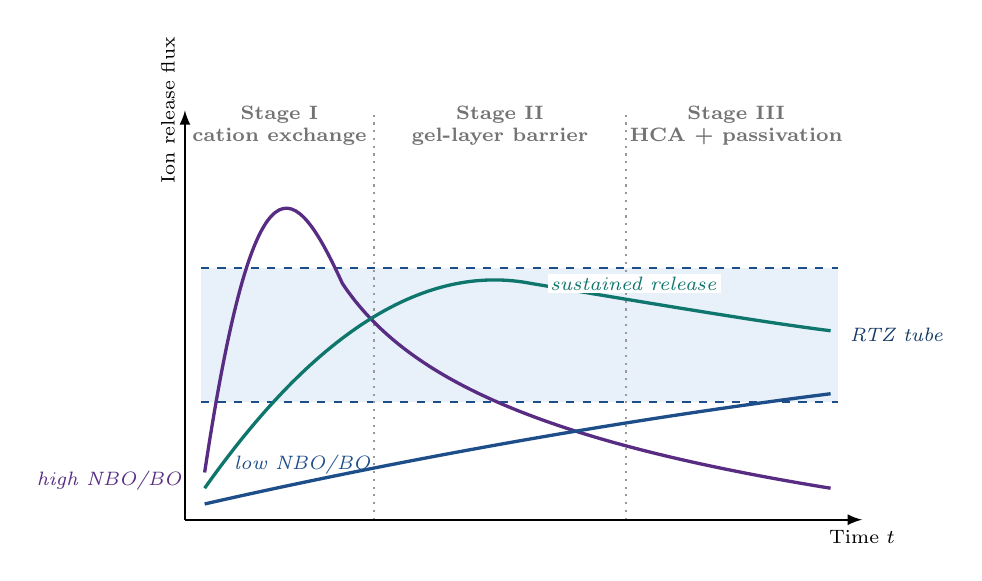
\begin{tikzpicture}[>=latex, font=\rmfamily, scale=1.0]

% 1. Background RTZ Tube
\fill[ukblue!70] (0.2,1.5) rectangle (8.3,3.2);
\draw[thick, dashed, chemblue] (0.2,1.5) -- (8.3,1.5);
\draw[thick, dashed, chemblue] (0.2,3.2) -- (8.3,3.2);
\node[anchor=west, font=\scriptsize, chemblue!75!black] at (8.32,2.35) {\emph{RTZ tube}};

% 2. Stage Separators (Vertical Dotted Lines)
\draw[thick, dotted, gray!80] (2.4, 0) -- (2.4, 5.2);
\draw[thick, dotted, gray!80] (5.6, 0) -- (5.6, 5.2);

% 3. Stage Labels (Centered within their respective time windows)
\node[font=\scriptsize\bfseries, gray!90!black, align=center] at (1.2, 5.0) {Stage I\\cation exchange};
\node[font=\scriptsize\bfseries, gray!90!black, align=center] at (4.0, 5.0) {Stage II\\gel-layer barrier};
\node[font=\scriptsize\bfseries, gray!90!black, align=center] at (7.0, 5.0) {Stage III\\HCA + passivation};

% 4. Axes
\draw[->, thick] (0,0) -- (8.6,0) node[below]{\scriptsize Time $t$};
\draw[->, thick] (0,0) -- (0,5.2) node[below, rotate=90, above]{\scriptsize Ion release flux};

% 5. Trajectory Curves
% High NBO/BO
\draw[very thick, statepurple] (0.25,0.6) .. controls (0.9,4.9) and (1.4,4.3) .. (2.0,3.0)
     .. controls (2.8,1.8) and (4.5,1.0) .. (8.2,0.4);
\node[anchor=east, font=\scriptsize, statepurple] at (0.1,0.5) {\emph{high NBO/BO}};

% Sustained Release
\draw[very thick, archgreen] (0.25,0.4) .. controls (1.1,1.6) and (2.6,3.35) .. (4.4,3.0)
     .. controls (6.2,2.7) and (7.4,2.5) .. (8.2,2.4);
\node[anchor=west, font=\scriptsize, archgreen, fill=white, inner sep=1pt] at (4.6,3 ) {\emph{sustained release}};

% Low NBO/BO
\draw[very thick, chemblue] (0.25,0.2) .. controls (2.0,0.6) and (5.0,1.2) .. (8.2,1.6);
\node[anchor=east, font=\scriptsize, chemblue] at (2.5,0.7 ) {\emph{low NBO/BO}};

\end{tikzpicture}
\caption{Chemical trajectory families generated by the network-energetics model of Section~\ref{sec:chem}. High-NBO/BO compositions produce a sharp anabolic burst followed by gel-layer-mediated passivation (overshoot risk); low-NBO/BO compositions deliver a flat, sub-threshold plateau (underdose risk); only intermediate networks sustain a release flux inside the Regenerative Target Zone (shaded band; Section~\ref{sec:biology}). The three labeled stages are the incongruent-dissolution windows of Section~\ref{sec:gel}.}
\label{fig:chem}
\end{figure}

%============================================================
% 3. ARCHITECTURAL TRAJECTORY ENGINEERING
%============================================================
\section{Architectural Trajectory Engineering: Pore-Network Design and Dynamic Transport Control}
\label{sec:arch}


The architectural layer is the \emph{transport term}: it determines how the source fluxes are dispersed, mixed, and convected into the tissue-facing space. We distinguish static architectural control (Section~\ref{sec:arch_static}) from the dynamic, degradation-induced reconfiguration of transport properties (Section~\ref{sec:arch_dynamic}), which requires the moving-boundary machinery of Section~\ref{sec:couple}.


\subsection{Additive Manufacturing as the Architectural Design Instrument}
\label{sec:arch_static}


Additive manufacturing (AM) has made pore architecture a \emph{first-class design variable}. Direct ink writing (DIW) \cite{Elsayed2017,Liu2021, Workie2023}, digital light processing (DLP) \cite{Elsayed2018,Napolitano2020}, stereolithography \cite{Chamhibrahim2025} and binder jetting \cite{Tang2022} deliver deterministic control of porosity, strut diameter, connectivity, anisotropy and spatial gradients. DIW of polymer-derived ceramics is of particular strategic value because the preceramic route decouples \emph{ink chemistry} (which encodes the trajectory) from \emph{print geometry} (which encodes the transport field) \cite{Colombo2010,Li2026}. Substantial work has validated this approach across wollastonite--diopside systems \cite{Elsayed2017}, Biosilicate \cite{Elsayed2019} and DIW-processed functionally graded bone scaffolds \cite{Furlan2026,Elsayed2021}, at porosity 40--75\%, struts 200--600~\si{\micro\meter}, and lattices from simple cubic to functionally graded \cite{Elsayed2021,Su2025}.


\subsection{Static Transport Metrics}


For a fixed (time-invariant) architecture, the effective diffusivity obeys the porosity--tortuosity scaling
\begin{equation}
\Veff \;=\; D_0\,\frac{\varepsilon}{\kappa^{2}}\,g(\varepsilon),
\label{eq:D_eff_static}
\end{equation}
where the percolation function $g(\varepsilon)$ vanishes below the percolation threshold and is commonly parametrized as $g(\varepsilon)=\varepsilon^{1/2}$ (Millington--Quirk), giving the widely used relation $\Veff/D_0\approx\varepsilon^{3/2}/\kappa^{2}$ \cite{Tjaden2016, Millington1959,Bruggeman1935}. Equation~\eqref{eq:D_eff_static} is the static limit of the dynamic law of Section~\ref{sec:arch_dynamic}. The geometric source-scaling factor at the scaffold level is the specific surface
\begin{equation}
\beta(\mathbf{x},0) \;=\; \frac{SA}{V} \;\simeq\; \frac{n_{\mathrm{struts}}\,\pi\,d_{\mathrm{strut}}\,l_{\mathrm{strut}}}{V_{\mathrm{scaffold}}},
\label{eq:beta_static}
\end{equation}
which for open cubic lattices with unit-cell edge $l$ and strut diameter $d\ll l$ reduces to $\beta\simeq3\pi d/(2l^{2})$ \cite{Liu2021}. Table~\ref{tab:arch} ranks canonical architectures by static transport metrics and, hence, by their \emph{intrinsic} trajectory class.


\begin{table}[htbp]
\centering
\caption{Canonical scaffold architectures, static transport metrics, and implied transport regime (computed at $D_0=1\times10^{-9}$\,m$^{2}$\,s$^{-1}$, perfusion velocity $U=10\,\mu$m\,s$^{-1}$, length scale $L=500\,\mu$m).}
\label{tab:arch}
\tablesize
\begin{tabular}{L{1.9cm} C{1.1cm} C{1.3cm} C{1.2cm} C{1.2cm} C{1.5cm} C{2.6cm}}
\toprule
\rowcolor{gray!12}
\textbf{Architecture} & $\varepsilon$ & $d_{\mathrm{strut}}$ ($\mu$m) & $\beta$ (cm$^{-1}$) & $\kappa$ & $\Veff/D_0$ & \textbf{Trajectory implication} \\
\midrule
Simple cubic & 0.55 & 400 & 42 & 1.15 & $\approx$0.44 & Homogeneous, fast equilibration \\
Hexagonal packed & 0.50 & 350 & 48 & 1.30 & $\approx$0.32 & Intermediate gradients \\
Gradient porosity & 0.40--0.70 & 200--600 & 30--150 & 1.1--1.6 & 0.18--0.65 & Programmed spatial gradients \\
Stochastic/foam & 0.65 & 250 & 65 & 1.60 & $\approx$0.40 & Heterogeneous, bio-mimetic \\
Woven/fiber & 0.50 & 300 & 55 & 1.50 (axial) & $\approx$0.25 & Directional transport \\
\bottomrule
\end{tabular}
\end{table}


\subsection{Degradation-Triggered Reconfiguration (Framework of Dynamic Metrics)}
\label{sec:arch_dynamic}


The architectural layer would be of limited interest if it were static. In reality, degradation continuously reconfigures the pore network: mass loss converts solid struts into receding cylinders, opens pores, lowers tortuosity, and raises $\Veff$ until structural collapse sets in. These coupled dynamics are governed by the moving-boundary laws derived next; the architectural terminology here becomes dynamic by writing
\begin{equation}
\Veff(\mathbf{x},t) \;=\; D_0\,\frac{\bigl[\varepsilon(\mathbf{x},t)\bigr]^{3/2}}{\bigl[\kappa(\mathbf{x},t)\bigr]^{2}},\qquad
\kappa(\mathbf{x},t) \;=\; \kappa_0\Bigl(\frac{\varepsilon(\mathbf{x},0)}{\varepsilon(\mathbf{x},t)}\Bigr)^{q},
\label{eq:D_eff_dynamic}
\end{equation}
with $q\in[0.3,1.0]$ an architecture-dependent exponent and $\kappa_0$ the pristine tortuosity. Equation~\eqref{eq:D_eff_dynamic} is the bridge Section~\ref{sec:couple} will close: once $\varepsilon(\mathbf{x},t)$ is known from the moving-boundary balance, the entire transport field is known and the state vector $\mathbf{S}(\mathbf{x},t)$ becomes computable.


%============================================================
% 4. MOVING-BOUNDARY COUPLED FRAMEWORK
%============================================================
\section{The Moving-Boundary Coupled Reactor: Porosity Evolution, Convective Transport and the Damk\"ohler--P\'eclet Regime Map}
\label{sec:couple}


The central assertion of this work is that chemistry and architecture cannot be designed separately: they are locked together by the moving reaction boundary and by the transport field that this same boundary reconfigures. This section upgrades the static reaction--diffusion statement into a closed, self-consistent, moving-boundary reactor model and derives its dimensionless regime structure.


\subsection{Porosity Evolution and the Moving-Boundary Law}


The porosity at point $\mathbf{x}$ increases because dissolving strut surfaces recede. From the surface-recession velocity \eqref{eq:recession} and mass conservation,
\begin{equation}
\pde{\varepsilon(\mathbf{x},t)}{t} \;=\; k^{\circ}_{\mathrm{diss}}\,\alpha(Q^n,t)\;\beta(\mathbf{x},t)\;\bar{V}_m,
\label{eq:eps_evol}
\end{equation}
where $\bar{V}_m=M_r/\rho_s$ is the network molar volume. This form is dimensionally consistent: $[\mathrm{mol\,m^{-2}s^{-1}}]\times[\mathrm{m^{-1}}]\times[\mathrm{m^{3}\,mol^{-1}}]=[\mathrm{s^{-1}}]$. For cylindrical struts the geometric factor closes the system:
\begin{equation}
\beta(\mathbf{x},t) \;=\; \frac{SA}{V} \;=\; \frac{3\,\bigl(1-\varepsilon(\mathbf{x},t)\bigr)}{r_s(\mathbf{x},t)},
\label{eq:beta_dyn}
\end{equation}
and Eqs.~\eqref{eq:eps_evol}--\eqref{eq:beta_dyn} together with \eqref{eq:recession} constitute the moving-boundary (erosion) law. Physically, Eq.~\eqref{eq:eps_evol} states that the trajectory's geometric degrees of freedom are not inputs but \emph{states}: every instant of degradation writes a new porosity field, which rewrites the transport field through Eq.~\eqref{eq:D_eff_dynamic}.


\begin{figure}[htbp]
\centering
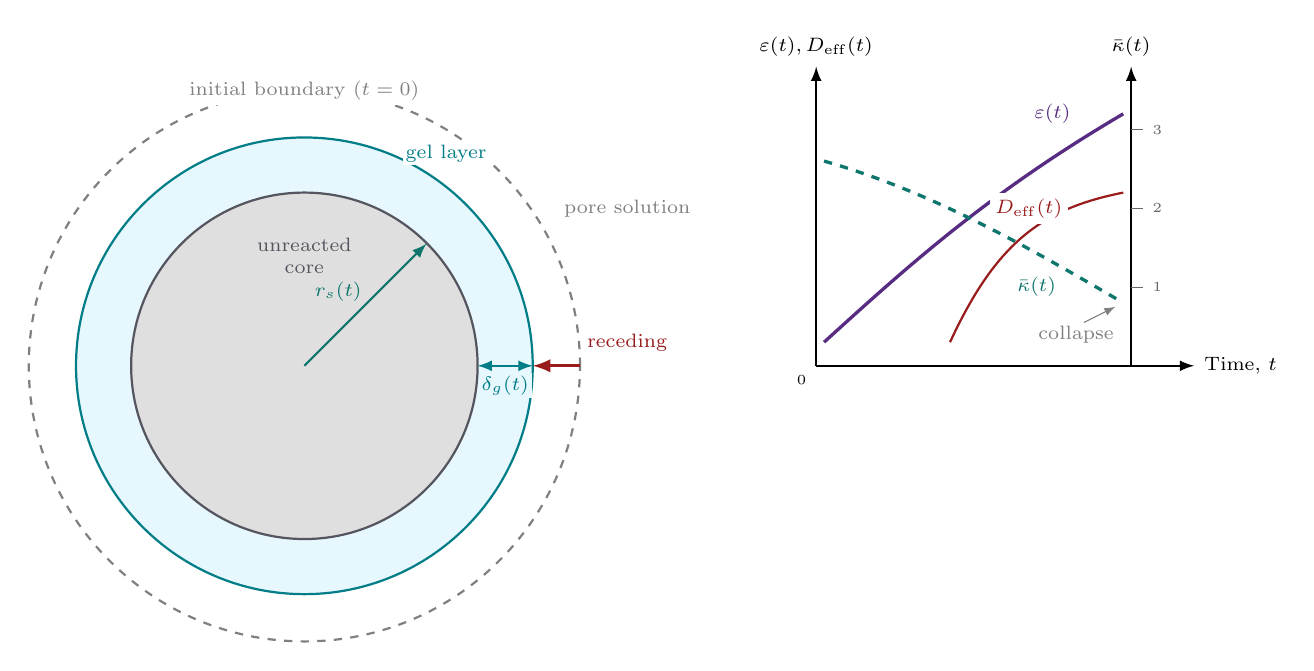
\begin{tikzpicture}[>=latex, font=\rmfamily, scale=1.0]

% ==========================================
% LEFT PANEL: Strut cross-section
% ==========================================
% Center anchor point
\fill[black!60] (0,0) circle (1.5pt);

% Initial state (t=0) - Gives the circles meaning as a "receding" boundary
\draw[thick, gray, dashed] (0,0) circle (3.5);
\node[font=\scriptsize, gray, fill=white, inner sep=2pt] at (0,3.5) {initial boundary ($t=0$)};

% Current gel layer (outer)
\draw[thick, gelcyan, fill=cyan!10] (0,0) circle (2.9);
\node[gelcyan, font=\scriptsize, fill=white, inner sep=1pt] at (1.8,2.7) {gel layer};

% Current unreacted core (inner)
\draw[thick, coregray, fill=gray!25] (0,0) circle (2.2);
\node[coregray, font=\scriptsize, align=center] at (0,1.4) {unreacted \\ core};

% Annotations for thickness and radius
\draw[<->, thick, gelcyan] (2.2,0) -- (2.9,0);
\node[gelcyan, font=\scriptsize, fill=cyan!10, inner sep=1pt] at (2.55,-0.25) {$\delta_g(t)$};

% Radius arrow from center
\draw[->, thick, archgreen] (0,0) -- (1.55, 1.55) node[midway, above left, font=\scriptsize, inner sep=1pt] {$r_s(t)$};

% Receding direction arrow
\draw[->, very thick, rtzred] (3.5,0) -- (2.9,0);
\node[rtzred, font=\scriptsize, fill=white, inner sep=2pt] at (4.1,0.3) {receding};
\node[font=\scriptsize, gray, fill=white, inner sep=2pt] at (4.1,2.0) {pore solution};


% ==========================================
% RIGHT PANEL: Porosity/Evolution Curve
% ==========================================
% Using a scope to reset coordinates to (0,0) for the graph, making it cleaner
\begin{scope}[xshift=6.5cm]
    
    % X-Axis
    \draw[->, thick] (0,0) -- (4.8,0) node[right, font=\scriptsize] {Time, $t$};
    \node[below left, font=\tiny] at (0,0) {0};
    
    % Left Y-axis (Porosity & Diffusivity)
    \draw[->, thick] (0,0) -- (0,3.8) node[above, font=\scriptsize] {$\varepsilon(t), \Veff(t)$};
    
    % Right Y-axis (Tortuosity)
    \draw[->, thick] (4.0,0) -- (4.0,3.8) node[above, font=\scriptsize] {$\bar{\kappa}(t)$};
    
    % Ticks for right axis
    \draw[black!60, thin] (4.0,1.0) -- (4.15,1.0) node[right, font=\tiny] {1};
    \draw[black!60, thin] (4.0,2.0) -- (4.15,2.0) node[right, font=\tiny] {2};
    \draw[black!60, thin] (4.0,3.0) -- (4.15,3.0) node[right, font=\tiny] {3};

    % Curves
    % Porosity \varepsilon(t)
    \draw[very thick, statepurple] (0.1,0.3) .. controls (1.2,1.3) and (2.2,2.2) .. (3.9,3.2);
    \node[statepurple, font=\scriptsize, fill=white, inner sep=2pt] at (3.0,3.2) {$\varepsilon(t)$};

    % Tortuosity \bar{\kappa}(t)
    \draw[very thick, archgreen, dashed] (0.1,2.6) .. controls (1.5,2.2) and (2.7,1.5) .. (3.9,0.8);
    \node[archgreen, font=\scriptsize, fill=white, inner sep=2pt] at (2.8,1 ) {$\bar{\kappa}(t)$};
    
    % Collapse indicator
    \node[font=\scriptsize, gray, fill=white, inner sep=2pt] at (3.3, 0.4) {collapse};
    \draw[->, gray, thin] (3.4, 0.55) -- (3.8, 0.75);

    % Effective Volume/Diffusivity \Veff(t)
    \draw[thick, rtzred] (1.7,0.3) .. controls (2.3,1.6) and (2.9,2.0) .. (3.9,2.2);
    \node[rtzred, font=\scriptsize, fill=white, inner sep=2pt] at (2.7,2) {$\Veff(t)$};

\end{scope}

\end{tikzpicture}
\caption{Moving-boundary erosion of a DIW strut (cross-section) and the resulting state-field evolution. The gel layer at the solid--solution interface bounds the released-ion flux (Eq.~\eqref{eq:gel_flux}); the receding radius $r_s(t)$ drives porosity growth (Eq.~\eqref{eq:eps_evol}); porosity and tortuosity jointly renormalize the effective diffusivity (Eq.~\eqref{eq:D_eff_dynamic}). The dashed falling curve indicates the eventual percolation-to-collapse limit in over-fast dissolution.}
\label{fig:moving}
\end{figure}


\subsection{The Coupled Master Equation for Ion Transport}


Superimposing (i) molecular diffusion with dynamic $\Veff(\mathbf{x},t)$, (ii) interstitial convection, and (iii) the chemistry--architecture source and HCA sink, yields the master equation
\begin{equation}
\pde{C_i}{t} \;+\; \underbrace{\nabla\!\cdot\!\bigl(\mathbf{u}\,C_i\bigr)}_{\text{convection}}
\;=\; \underbrace{\nabla\!\cdot\!\Bigl[\Veff(\mathbf{x},t)\,\nabla C_i\Bigr]}_{\text{diffusion}}
\;+\; \underbrace{k^{\circ}_{\mathrm{diss},i}\,\alpha(Q^n,t)\,\beta(\mathbf{x},t)\,\phi(\SIhc)}_{\text{source: chemistry}\times\text{architecture}}
\;-\; \underbrace{k_{\mathrm{precip},i}\,\gamma(\SIhc)}_{\text{precipitation sink}},
\label{eq:master}
\end{equation}
with the reaction--diffusion modifiers
\begin{equation}
\phi(\SIhc)=1-e^{-\SIhc^{2}},\qquad
\gamma(\SIhc)=\max\!\Bigl(0,\;1-e^{-(\SIhc-\SIhc^{\mathrm{crit}})}\Bigr),
\label{eq:phi_gamma}
\end{equation}
$\SIhc^{\mathrm{crit}}$ being the critical saturation index for precipitation onset. Equation~\eqref{eq:master} is closed by the coupled set \eqref{eq:eps_evol}, \eqref{eq:beta_dyn}, \eqref{eq:D_eff_dynamic}, \eqref{eq:ph_feedback} and the gel-layer flux \eqref{eq:gel_flux}. It is \emph{moving-boundary} because the domain conductivity, source, and sink all inherit the porosity evolution; it is \emph{multi-species} because $i\in\{\mathrm{Ca,Si,Mg}\}$ exchange mass through HCA stoichiometry and the pH feedback \eqref{eq:ph_feedback}; and it is \emph{open-loop controllable} because the controllable inputs (composition $\rightarrow\alpha$, geometry $\rightarrow\beta_0$) enter only in the initial and boundary data.


\subsection{Interstitial Convective Transport: The Brinkman Layer}


In vivo, the scaffold pore space is perfused by interstitial fluid, and trajectory fidelity requires modeling convection as porous-medium flow rather than free Stokes flow. The monophasic \emph{Brinkman} extension of Darcy's law \cite{Brinkman1947,Bear1972} supplies the momentum balance
\begin{equation}
-\nabla p + \mu_{\mathrm{eff}}\,\nabla^{2}\mathbf{u} - \frac{\mu}{\kappa_m\bigl(\varepsilon(\mathbf{x},t)\bigr)}\,\mathbf{u} = 0,\qquad
\nabla\!\cdot\!\mathbf{u}=0,
\label{eq:brinkman}
\end{equation}
with Darcy permeability evolving with porosity (e.g., Kozeny--Carman, $\kappa_m\propto\varepsilon^{3}/(1-\varepsilon)^{2}$). The coupled system \eqref{eq:master}--\eqref{eq:brinkman} recovers the classical limits: $\mu_{\mathrm{eff}}\!\to\!0$ gives pure Darcy flow; $\kappa_m\!\to\!\infty$ gives Stokes (free-fluid) convection. Importantly, as degradation raises $\varepsilon$, it simultaneously raises $\kappa_m$ and $\Veff$, so the \emph{flow field itself is trajectory-coupled}, the spatial distribution of delivered ions changes as the scaffold partially resorbs.


\subsection{Dimensionless Regime Structure: The Damk\"ohler--P\'eclet Map}


Nondimensionalizing Eqs.~\eqref{eq:master}--\eqref{eq:brinkman} with length scale $L$, velocity $U$, diffusion time $L^{2}/\Veff$ and reaction time $1/(k^{\circ}_{\mathrm{diss}}\alpha\beta)$ yields two governing numbers:
\begin{equation}
\mathrm{Da} \;=\; \frac{k^{\circ}_{\mathrm{diss}}\,\alpha\,\beta\,L^{2}}{\Veff}\quad\text{(reaction/diffusion)},\qquad
\mathrm{Pe} \;=\; \frac{U\,L}{\Veff}\quad\text{(convection/diffusion)}.
\label{eq:Da_Pe}
\end{equation}


The $(\log\mathrm{Da},\log\mathrm{Pe})$ plane partitions into four phenomenologically distinct quadrants plus a coupled design corridor (Table~\ref{tab:regimes} and Fig.~\ref{fig:dape}):


\begin{itemize}[leftmargin=1.5em,itemsep=1pt]
\item \textbf{Q1} ($\mathrm{Da}\ll1$, $\mathrm{Pe}\ll1$): \emph{reaction-limited, diffusion-dominated}. Slow release, nearly homogeneous, gentle plateaus; safe but frequently sub-threshold (underdose).
\item \textbf{Q2} ($\mathrm{Da}\gg1$, $\mathrm{Pe}\ll1$): \emph{diffusion-limited}. Fast surface release cannot be dispersed; steep boundary layers, local supersaturation, HCA overshoot and passivation; the classic ``burst then silence'' failure mode, with cytotoxic spike risk.
\item \textbf{Q3} ($\mathrm{Da}\ll1$, $\mathrm{Pe}\gg1$): \emph{convective washout}. Released ions are convected away faster than they accumulate; systemic dilution and minimal local osteogenic drive.
\item \textbf{Q4} ($\mathrm{Da}\gg1$, $\mathrm{Pe}\gg1$): \emph{convection-amplified localized dosing}. Rapid release delivered downstream; steep gradients and progressive loss of mechanical integrity.
\item \textbf{Design corridor} ($\mathrm{Da}\sim1$, $\mathrm{Pe}\sim1$): the coupled window where reaction and transport compete and neither alone predicts the trajectory, the region where trajectory classes diverge maximally, and where the RTZ (Section~\ref{sec:biology}) is expected to be populated.
\end{itemize}


Equation~\eqref{eq:Da_Pe} states the decisive design conclusion of this work: the chemical knob ($\alpha$, through $Q^n$) and the architectural knobs ($\beta$, $\Veff$, through $\varepsilon,\kappa$) are \emph{non-separable} because both enter $\mathrm{Da}$. Static composition--geometry screening cannot relocate a design from Q2 into the corridor without changing $\mathrm{Da}$; only simultaneous, coupled chemistry--architecture engineering can. This is the mathematical content of trajectory engineering.


 \begin{table}[htbp]
\centering
\caption{Damk\"ohler--P\'eclet regime analysis for trajectory class prediction. Boundary values are nominal; exact thresholds depend on the ion, scaffold and implantation site.}
\label{tab:regimes}
\tablesize
\begin{tabular}{L{1.9cm} C{1.5cm} C{1.5cm} L{4.3cm} L{3.0cm} L{2.4cm}}
\toprule
\rowcolor{gray!12}
\textbf{Regime} & $\mathrm{Da}$ & $\mathrm{Pe}$ & \textbf{Mechanism} & \textbf{Trajectory class} & \textbf{Risk} \\
\midrule
Q1 & $\ll1$ & $\ll1$ & Reaction-limited, homogeneous diffusion & Slow plateau below RTZ & Underdose \\
Q2 & $\gg1$ & $\ll1$ & Diffusion-limited boundary layer & Burst $\rightarrow$ passivation & Overdose spike \\
Q3 & $\ll1$ & $\gg1$ & Convective washout & Dilute, spatially uniform & Bioinert \\
Q4 & $\gg1$ & $\gg1$ & Convection-amplified dosing & Steep downstream gradients & Erosion / SI loss \\
\textbf{Corridor} & $\sim1$ & $\sim1$ & Coupled reaction--transport & RTZ-populated, class divergence & --- \\
\bottomrule
\end{tabular}
\end{table}

\vspace{0.8em}

\begin{figure}[htbp]
\centering
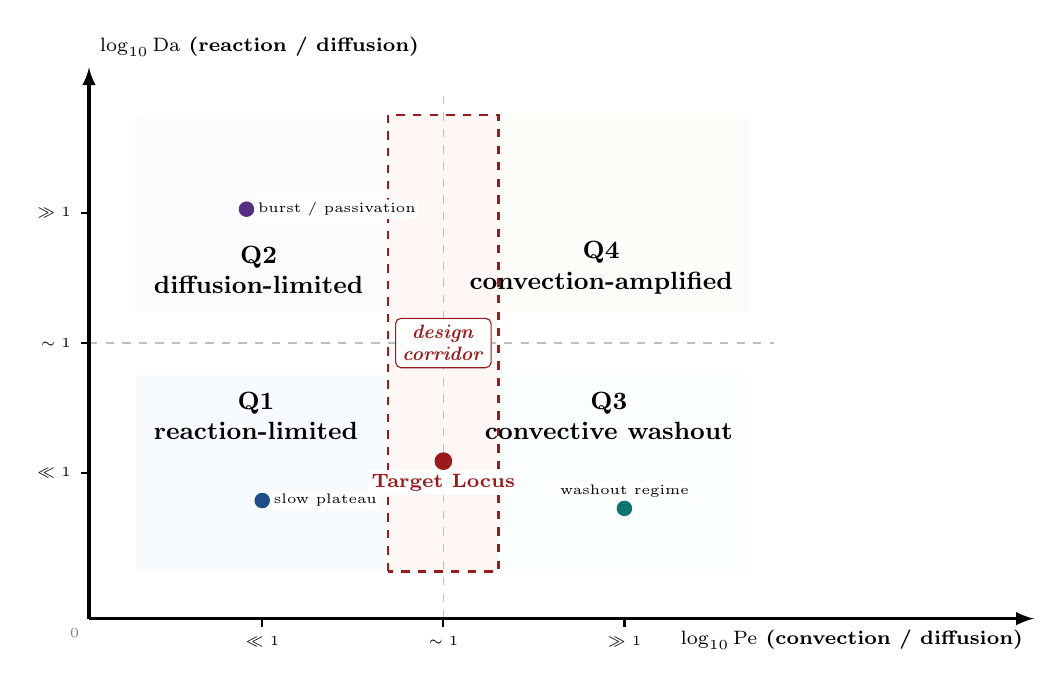
\begin{tikzpicture}[>=latex, font=\rmfamily, scale=1.0]

% ==========================================
% Quadrant Background Fills
% ==========================================
% Q1: Bottom-Left
\fill[ukblue!20] (0.6, 0.6) rectangle (3.8, 3.1);
% Q2: Top-Left
\fill[ukpurple!20] (0.6, 3.9) rectangle (3.8, 6.4);
% Q3: Bottom-Right
\fill[ukgreen!20] (5.2, 0.6) rectangle (8.4, 3.1);
% Q4: Top-Right
\fill[ukamber!20] (5.2, 3.9) rectangle (8.4, 6.4);

% Central Design Corridor Fill (Da ~ 1, Pe ~ 1)
\fill[ukred!30, draw=rtzred, thick, dashed] (3.8, 0.6) rectangle (5.2, 6.4);

% ==========================================
% Grid Reference Lines (Center at Pe=1, Da=1)
% ==========================================
\draw[gray!50, dashed] (4.5, 0) -- (4.5, 6.7);
\draw[gray!50, dashed] (0, 3.5) -- (8.7, 3.5);

% ==========================================
% Main Axes & Ticks
% ==========================================
% X-axis
\draw[->, very thick] (0,0) -- (12.0,0) node[below left, font=\scriptsize\bfseries] {$\log_{10}\mathrm{Pe}$ (convection / diffusion)};
\draw[thick] (2.2,0) -- (2.2,-0.1) node[below, font=\tiny] {$\ll 1$};
\draw[thick] (4.5,0) -- (4.5,-0.1) node[below, font=\tiny] {$\sim 1$};
\draw[thick] (6.8,0) -- (6.8,-0.1) node[below, font=\tiny] {$\gg 1$};

% Y-axis
\draw[->, very thick] (0,0) -- (0,7.0) node[above right, font=\scriptsize\bfseries] {$\log_{10}\mathrm{Da}$ (reaction / diffusion)};
\draw[thick] (0,1.85) -- (-0.1,1.85) node[left, font=\tiny] {$\ll 1$};
\draw[thick] (0,3.5)  -- (-0.1,3.5)  node[left, font=\tiny] {$\sim 1$};
\draw[thick] (0,5.15) -- (-0.1,5.15) node[left, font=\tiny] {$\gg 1$};

% Origin tag
\node[below left, font=\tiny, gray] at (0,0) {0};

% ==========================================
% Quadrant Labels (Positioned in Corners)
% ==========================================
\node[font=\small\bfseries, align=center, anchor=north west] at (0.7, 3.0) {Q1\\reaction-limited};
\node[font=\small\bfseries, align=center, anchor=south west] at (0.7, 4.0) {Q2\\diffusion-limited};
\node[font=\small\bfseries, align=center, anchor=north east] at (8.3, 3.0) {Q3\\convective washout};
\node[font=\small\bfseries, align=center, anchor=south east] at (8.3, 4.0) {Q4\\convection-amplified};

% Design Corridor Badge Label
\node[font=\scriptsize\bfseries, rtzred, align=center, fill=white, draw=rtzred, rounded corners=2pt, inner sep=2.5pt] at (4.5, 3.5) {\emph{design}\\\emph{corridor}};

% ==========================================
% Loci / Data Points (Cleanly Offset from Text)
% ==========================================
% Point in Q2
\fill[statepurple] (2.0, 5.2) circle (2.8pt);
\node[right=3pt, font=\tiny, fill=white, inner sep=1pt, rounded corners=1pt] at (2.0, 5.2) {burst / passivation};

% Point in Q1
\fill[chemblue] (2.2, 1.5) circle (2.8pt);
\node[right=3pt, font=\tiny, fill=white, inner sep=1pt, rounded corners=1pt] at (2.2, 1.5) {slow plateau};

% Point in Q3
\fill[archgreen] (6.8, 1.4) circle (2.8pt);
\node[above=3pt, font=\tiny, fill=white, inner sep=1pt, rounded corners=1pt] at (6.8, 1.4) {washout regime};

% Target Locus in Design Corridor
\fill[rtzred] (4.5, 2.0) circle (3.2pt);
\node[below=3pt, font=\scriptsize\bfseries, rtzred, fill=white, inner sep=1.5pt] at (4.5, 2.0) {Target Locus};

\end{tikzpicture}
\caption{Damk\"ohler--P\'eclet regime map for the moving-boundary reactor (Eqs.~\eqref{eq:master}--\eqref{eq:Da_Pe}). Points are computed trajectory loci for representative compositions and architectures; the shaded corridor ($\mathrm{Da}\sim1$, $\mathrm{Pe}\sim1$) is the coupled region where trajectory classes diverge maximally and the Regenerative Target Zone is expected to be populated. Trajectory engineering is the operation of relocating designs into this corridor through joint chemistry--architecture control.}
\label{fig:dape}
\end{figure}


\subsection{Spatiotemporal Consistency and the State Vector}


Integrating Eqs.~\eqref{eq:eps_evol}--\eqref{eq:Da_Pe}, the state vector becomes a piecewise smooth function of space and time:
\begin{equation}
\mathbf{S}(\mathbf{x},t)=\Bigl[C_{\mathrm{Ca}},\,C_{\mathrm{Si}},\,C_{\mathrm{Mg}},\,\mathrm{pH},\,\varepsilon,\,D_{\mathrm{eff}}\Bigr]^{T}\!\in\mathbb{R}^{6},\qquad
\frac{\dd \mathbf{S}}{\dd t}=\mathcal{F}\bigl(\mathbf{S},\boldsymbol{\theta}\bigr),
\label{eq:state_ode}
\end{equation}
where $\mathcal{F}$ is the reduced vector field induced by the PDE system and $\boldsymbol{\theta}$ collects the material parameters. Equation~\eqref{eq:state_ode} is written in ODE-in-time form deliberately because it is the object that Section~\ref{sec:comp} learns from data via neural ODEs, and the residual constraint that physics-informed neural networks embed.


%============================================================
% 5. BIOLOGICAL VALIDATION AND THE RTZ
%============================================================
\section{Biological Validation and the Regenerative Target Zone as a Continuous Admissibility Tube}
\label{sec:biology}


Static endpoint criteria (``ALP$\geq2\times$ at Day 14, M2/M1$\geq3\times$ at Day 7, mineralization$\geq50\%$ at Day 28'') are useful checkpoints, but they are epistemically insufficient: they test the trajectory at isolated instants and can be satisfied by biologically divergent profiles. This section replaces them with a \emph{continuous} admissibility tube and supplies the temporally resolved osteo-immunomodulatory kinetics the tube encodes.


\subsection{The Tissue-Level Phase Architecture}


Bone regeneration is a phase-structured immune--skeletal program. We formalize it as three operational phases, parameterized by the state vector $\mathbf{S}(t)$ local to the implantation site \cite{Tian2022,Liu2024,Miron2016}:


\paragraph{Phase I ($0<t\leq48$\,h): the M1-gated inflammation window.}
Acute, spatially confined M1 signaling (TNF-$\alpha$, IL-1$\beta$, IL-6, iNOS) performs debris clearance, modulates the provisional fibrin scaffold, and recruits circulating osteo-chondrogenic progenitors (SDF-1$\alpha$/CXCR4 axis) \cite{Miron2016,Francois2018}. This window is \emph{gating}: its absence (complete bio-inertness) abolishes the downstream regenerative program, while excessive or prolonged M1 activity drives fibrous encapsulation. The trajectory constraint at this stage is a \emph{ceiling} on ion flux that prevents uncontrolled necrosis and an alkaline over-shock \cite{Polo-Montalvo2021}.


\paragraph{Phase II (Days 3--7): the controlled M1$\rightarrow$M2 transition.}
Pro-regenerative M2 polarization (Arg-1, CD206, IL-10, TGF-$\beta$1) is driven by Ca$^{2+}$/Si$^{4+}$/Mg$^{2+}$ flux falling into a narrow sustained band \cite{Polo-Montalvo2021,Zhang2021}. The transition defines the \emph{immunological switch}: the M2/M1 ratio must climb to $\geq3$ by Day 7 and persist. Trajectories that overshoot the band (Q2/Q4 regimes) re-ignite M1 signaling; trajectories that undershoot (Q1/Q3) fail to recruit and sustain osteoprogenitors.


\paragraph{Phase III ($t\gtrsim$Day 14): HCA maturation and osteogenic consolidation.}
HCA precipitation (Eq.~\eqref{eq:SI}) proceeds to mineralization fronts; ALP, RUNX2, OCN and OPN expression rises, and mineralized nodule area must reach $\geq50\%$ of the scaffold surface by Day 28, while remaining porosity holds above the percolation threshold to sustain vascular infiltration \cite{Xynos2000,Workie2023}.


\subsection{The Continuous Admissibility Tube (RTZ Envelope)}


We replace the discrete threshold set by a time-indexed \emph{envelope}---a tube in state space:
\begin{equation}
\RZT(t) \;=\; \Bigl\{\, \mathbf{S}(\cdot)\in C^{0}\bigl([0,T];\mathbb{R}^{6}\bigr) \;\Big|\;
C_{i}^{\min}(t)\leq C_{i}(t)\leq C_{i}^{\max}(t),\;\;
[\ce{H+}](t)\in[\ce{H+}]^{\mathrm{lo},\mathrm{hi}},\;\;
\varepsilon(t)\geq\varepsilon^{\mathrm{perc}},\;\;\forall\,t\in(0,T] \Bigr\},
\label{eq:rtz_tube}
\end{equation}
with $T$ the device end-of-life horizon and $\varepsilon^{\mathrm{perc}}$ the percolation threshold for open porosity. Membership is decided by the maximal tube distance
\begin{equation}
d_{\RZT}\bigl(\mathbf{S}\bigr) \;=\; \max_{t\in[0,T]}\bigl\Vert\mathbf{S}(t)-\Pi_{\RZT}(\mathbf{S}(t))\bigr\Vert_{2},\qquad
\mathbf{S}\in\RZT \iff d_{\RZT}(\mathbf{S})\leq\delta^{*},
\label{eq:tube_dist}
\end{equation}
where $\Pi_{\RZT}$ is the orthogonal projection onto the admissible tube and $\delta^{*}$ a tolerance. Equation~\eqref{eq:rtz_tube} is a genuine design specification: continuous, falsifiable, computable from Eq.~\eqref{eq:master}, and testable experimentally by longitudinal sampling. Table~\ref{tab:phases} lists phase-indexed tube bounds derived from published dose--response data.


\begin{table}[htbp]
\centering
\caption{Phase-indexed Regenerative Target Zone tube bounds. Criteria are derived from published dose, response data, and preclinical calibrations; recommended starting values for Bayesian recalibration (Section~\ref{sec:comp}).}
\label{tab:phases}
\tablesize
\begin{tabular}{L{2.6cm} C{1.3cm} C{2.2cm} C{3.4cm} C{3.0cm} C{2.0cm}}
\toprule
\rowcolor{gray!12}
\textbf{Phase} & \textbf{Window} & \textbf{Immunological program} & \textbf{Ion tube (band)} & \textbf{Molecular markers} & \textbf{Gate} \\
\midrule
I: Inflammation & 0--48\,h & M1 gating (clearance/recruitment) & $[\mathrm{Ca}]<8$\,mM; pH$<8.5$ & TNF-$\alpha$, IL-1$\beta$, IL-6, iNOS & $\varepsilon\geq\varepsilon^{\mathrm{perc}}$ \\
II: Transition & D3--D7 & M1$\rightarrow$M2 switch & Ca$^{2+}$ 1.5--6\,mM; Si(OH)$_4$ 10--40\,ppm; Mg$^{2+}$ 0.5--2\,mM & Arg-1, CD206, IL-10, TGF-$\beta$1; M2/M1$\geq3$ & $\varepsilon\geq\varepsilon^{\mathrm{perc}}$ \\
III: Maturation & $>$D14 & Osteogenic consolidation & sustained mid-band, decaying envelope & ALP, RUNX2, OCN, OPN; nodule$\geq50\%$ & $E(t)\geq E_{\min}$ \\
\bottomrule
\end{tabular}
\end{table}


\subsection{Phase-Kinetic Specification of the Tube}


The envelope \eqref{eq:rtz_tube} is fully realized only when its bounds encode the phase kinetics. Let $t_1=48$\,h and $t_2=7$\,d, and let $\Omega_k(t)$ ($k=\mathrm{I,II,III}$) be smoothed indicator weights with $\sum_k\Omega_k(t)=1$. Then the tube bounds decompose as
\begin{equation}
C_{i}^{\min}(t)=\sum_{k}\Omega_k(t)\,C_{i,k}^{\min},\qquad
C_{i}^{\max}(t)=\sum_{k}\Omega_k(t)\,C_{i,k}^{\max},
\label{eq:tube_phase}
\end{equation}
$\{C_{i,k}^{\min/\max}\}$ being the phase-constant bounds of Table~\ref{tab:phases}. This makes the RTZ a \emph{scheduled control specification} rather than a statistic: the design problem becomes ``find $(\alpha,\beta_0)$ such that the trajectory \eqref{eq:master} satisfies Eqs.~\eqref{eq:rtz_tube}--\eqref{eq:tube_phase}.'' We emphasize that the $\Omega_k(t)$ boundaries carry biological uncertainty; the Bayesian calibration of Section~\ref{sec:comp} treats $t_1$, $t_2$, and all bounds as random variables, yielding posterior \emph{credible tubes}.


\subsection{Experimental Validation Strategy}

Because Eq.~\eqref{eq:rtz_tube} is a functional hypothesis, its validation must be functional rather than endpoint-based:

\begin{enumerate}[leftmargin=1.6em]
\item \textbf{Longitudinal sampling:} ion release (ICP-OES), pH (SNARF-4F / microdialysis), porosity and $\Veff$ ($\mu$CT + tracer/EIS) at $\geq8$ timepoints across $[0,28]$\,d with $n\geq3$ replicate scaffolds \cite{Workie2026c,Elsayed2017}.
\item \textbf{Dynamic biological readouts:} time-resolved M1/M2 flow cytometry or qPCR; ALP and nodule area at multiple instants rather than single endpoints \cite{Workie2023,Polo-Montalvo2021}.
\item \textbf{Tube regression:} fit trajectory descriptors (peak height, time-to-peak, dose-rate envelope, tube distance \eqref{eq:tube_dist}) to the dynamic biological readouts; retain the trajectory descriptors as predictors and demonstrate that RTZ membership predicts outcome \emph{better} than any single static endpoint.
\end{enumerate}

% ============================================================
% FIGURE 4: Fixed in-place under Section 5.4
% ============================================================
\begin{figure}[H]
\centering
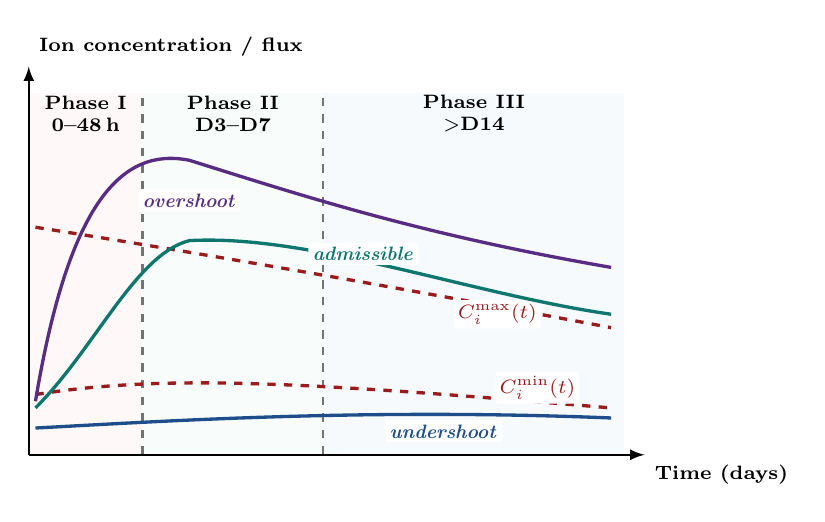
\begin{tikzpicture}[>=latex, font=\rmfamily, scale=0.85]

% Background phase panels
\fill[ukred!25] (0.,0.) rectangle (1.7,5.4);
\fill[ukgreen!30] (1.7,0.) rectangle (4.4,5.4);
\fill[ukblue!25] (4.4,0.) rectangle (8.9,5.4);

% Phase dividers
\draw[dashed, black!55, thick] (1.7,0) -- (1.7,5.4);
\draw[dashed, black!55, thick] (4.4,0) -- (4.4,5.4);

% Phase labels
\node[font=\scriptsize\bfseries, align=center] at (0.85,5.1) {Phase I\\ 0--48\,h};
\node[font=\scriptsize\bfseries, align=center] at (3.05,5.1) {Phase II\\ D3--D7};
\node[font=\scriptsize\bfseries, align=center] at (6.65,5.1) {Phase III\\ $>$D14};

% Tube Bounds (Red Dashed)
\draw[very thick, dashed, rtzred] (0.1,0.9) .. controls (2.0,1.2) and (4.0,1.1) .. (8.7,0.7);
\draw[very thick, dashed, rtzred] (0.1,3.4) .. controls (2.0,3.1) and (5.0,2.6) .. (8.7,1.9);

\node[rtzred, font=\scriptsize\bfseries, fill=white, inner sep=1.5pt, rounded corners=1pt] at (7.6,1.0) {$C_{i}^{\min}(t)$};
\node[rtzred, font=\scriptsize\bfseries, fill=white, inner sep=1.5pt, rounded corners=1pt] at (7.0,2.1) {$C_{i}^{\max}(t)$};

% Trajectories
% 1. Admissible (Green)
\draw[very thick, archgreen] (0.1,0.7) .. controls (1.0,1.6) and (1.6,3.0) .. (2.4,3.2)
     .. controls (4.2,3.3) and (6.6,2.4) .. (8.7,2.1);
\node[archgreen, font=\scriptsize\bfseries, fill=white, inner sep=1.5pt, rounded corners=1pt] at (5,3) {\emph{admissible}};

% 2. Overshoot (Purple)
\draw[very thick, statepurple] (0.1,0.8) .. controls (0.6,3.8) and (1.4,4.6) .. (2.4,4.4)
     .. controls (4.0,3.9) and (5.8,3.3) .. (8.7,2.8);
\node[statepurple, font=\scriptsize\bfseries, fill=white, inner sep=1.5pt, rounded corners=1pt] at (2.4,3.8) {\emph{overshoot}};

% 3. Undershoot (Blue)
\draw[very thick, chemblue] (0.1,0.4) .. controls (2.0,0.5) and (5.0,0.7) .. (8.7,0.55);
\node[chemblue, font=\scriptsize\bfseries, fill=white, inner sep=1.5pt, rounded corners=1pt] at (6.2,0.35) {\emph{undershoot}};

% Axes
\draw[->, thick] (0,0) -- (9.2,0) node[below right, font=\scriptsize\bfseries] {Time (days)};
\draw[->, thick] (0,0) -- (0,5.8) node[above right, font=\scriptsize\bfseries] {Ion concentration / flux};

\end{tikzpicture}
\caption{The Regenerative Target Zone as a continuous admissibility tube (Eqs.~\eqref{eq:rtz_tube}--\eqref{eq:tube_phase}). The three shaded panels are the osteo-immunomodulatory phases; the dashed red curves are the time-indexed tube bounds $C_{i}^{\min/\max}(t)$. Only trajectories that remain inside the tube for all $t\in[0,T]$, satisfying the phase-scheduled M1 gating, M2 switch, and maturation criteria, are RTZ-admissible. Static endpoint tests cannot distinguish the three trajectories; tube membership can.}
\label{fig:rtz}
\end{figure}

\FloatBarrier



%============================================================
% 6. ADVANCED COMPUTATIONAL MACHINERY
%============================================================
\section{Advanced Computational Machinery: Functional Data Analysis, Neural ODEs, Physics-Informed Neural Networks, and Bayesian Optimal Design}
\label{sec:comp}


The moving-boundary model of Section~\ref{sec:couple} and the tube constraint of Section~\ref{sec:biology} are only useful if their parameters can be estimated from real data, their predictions propagated with quantified uncertainty, and their observational campaigns designed to minimize that uncertainty. This section upgrades the pipeline accordingly.


\subsection{Functional Data Analysis and the End of Discrete-Endpoint Injection}


A trajectory is a \emph{curve}, not a vector of endpoint readings; standard PCA on time-sampled vectors discards the derivatives $\dd\mathbf{S}/\dd t$ that encode dose-rate, the most biologically decisive trajectory feature. Two tools from functional data analysis repair this.


\subsubsection{Functional Principal Component Analysis (fPCA)}
Let $\mu(t)=\mathbb{E}[\mathbf{S}(t)]$ and $\Sigma(s,t)=\mathrm{Cov}(\mathbf{S}(s),\mathbf{S}(t))$ be the mean and covariance functions estimated from the experimental trajectory population. Solving the functional eigenequation
\begin{equation}
\int_{0}^{T}\Sigma(s,t)\,\psi_k(t)\,\dd t \;=\; \lambda_k\,\psi_k(s),
\label{eq:fpca_eig}
\end{equation}
yields orthonormal eigenfunctions $\{\psi_k\}$ (the \emph{principal modes of variation} of the trajectories). The $k$-th functional score of a trajectory is the projection
\begin{equation}
\xi_k \;=\; \int_{0}^{T}\bigl(\mathbf{S}(t)-\mu(t)\bigr)\,\psi_k(t)\,\dd t,
\label{eq:fpca_score}
\end{equation}
and the parsimonious reconstruction
\begin{equation}
\mathbf{S}(t)\;\approx\; \mu(t)+\sum_{k=1}^{K}\xi_k\,\psi_k(t),\qquad K\ll N,
\label{eq:fpca_rec}
\end{equation}
retains essentially all trajectory information, including temporal derivatives, in a handful of scores \cite{Ramsay2009}. fPCA therefore compresses an entire dissolution--degradation campaign into a low-dimensional, biologically interpretable coordinate system---ideal input for the RTZ classifier.


\subsubsection{Dynamic Time Warping (DTW)}
For similarity assessment and clustering, DTW aligns two trajectories, allowing monotone local stretches and compressions, with cumulative cost
\begin{equation}
\mathcal{D}(i,j)\;=\;\min\!\bigl\{\mathcal{D}(i-1,j),\;\mathcal{D}(i,j-1),\;\mathcal{D}(i-1,j-1)\bigr\}\;+\;d\bigl(\mathbf{S}_i,\hat{\mathbf{S}}_j\bigr),
\label{eq:dtw}
\end{equation}
where $d(\cdot,\cdot)$ is a pointwise distance and $i,j$ index sample times of the two curves \cite{Sakoe1978}. DTW gives a rate-invariant distance that treats ``fast-then-slow'' and ``slow-then-fast'' profiles as distinct only when their warped shapes differ---exactly the invariance the biological outcome cares about (a plateau of any duration that stays in-band is acceptable; the same total dose delivered as a spike is not).


\subsection{Learning the Continuous Vector Field: Neural ODEs and PINNs}


\subsubsection{Neural Ordinary Differential Equations}
Given sparse dissolution and $\mu$CT data, we learn the reduced vector field of Eq.~\eqref{eq:state_ode} directly. A neural ODE parameterizes
\begin{equation}
\frac{\dd\mathbf{S}}{\dd t} \;=\; F_{\boldsymbol{\theta}}\bigl(\mathbf{S}(t),t\bigr),\qquad
\mathbf{S}(t_1)\;=\;\mathbf{S}(t_0)+\int_{t_0}^{t_1}F_{\boldsymbol{\theta}}\,\dd t,
\label{eq:node}
\end{equation}
where the integral is evaluated by an adaptive ODE solver and $F_{\boldsymbol{\theta}}$ is a neural network \cite{Chen2018}. Gradients with respect to $\boldsymbol{\theta}$ are obtained by the adjoint method: letting $\mathbf{a}(t)=\partial \mathcal{L}/\partial \mathbf{S}(t)$,
\begin{equation}
\frac{\dd\mathbf{a}}{\dd t} \;=\; -\mathbf{a}^{T}\,\frac{\partial F_{\boldsymbol{\theta}}}{\partial \mathbf{S}},\qquad
\frac{\dd \mathcal{L}}{\dd \boldsymbol{\theta}} \;=\; -\int_{t_1}^{t_0}\mathbf{a}^{T}\,\frac{\partial F_{\boldsymbol{\theta}}}{\partial \boldsymbol{\theta}}\,\dd t,
\label{eq:adjoint}
\end{equation}
which resolves the memory problem of backpropagating through ODE solvers. A calibrated neural ODE provides continuous-time posterior trajectory samples, the natural engine for Monte Carlo evaluation of the tube membership probability $\Pr(\mathbf{S}\in\RZT\mid\mathcal{D})$.


\subsubsection{Physics-Informed Neural Networks (PINNs)}
Where the governing PDE structure \eqref{eq:master}--\eqref{eq:brinkman} is trusted but parameters are uncertain, PINNs embed the physics as a soft residual constraint \cite{Raissi2019}. The surrogate $\hat{\mathbf{S}}_{\boldsymbol{\theta}}(\mathbf{x},t)$ is trained on the composite loss
\begin{equation}
\mathcal{L}(\boldsymbol{\theta}) \;=\; \lambda_D\mathcal{L}_{\mathrm{data}} + \lambda_P\mathcal{L}_{\mathrm{PDE}} + \lambda_B\mathcal{L}_{\mathrm{BC/IC}},
\label{eq:pinn_loss}
\end{equation}
\begin{equation}
\mathcal{L}_{\mathrm{PDE}} \;=\; \Bigl\|\pde{\hat{\mathbf{S}}}{t} + \nabla\!\cdot\!\bigl(\mathbf{u}\hat{\mathbf{S}}\bigr) - \nabla\!\cdot\!\bigl(\Veff(\mathbf{x},t)\nabla\hat{\mathbf{S}}\bigr) - \hat{\mathcal{R}}\Bigr\|^{2},
\label{eq:pinn_pde}
\end{equation}
where $\hat{\mathcal{R}}$ collects the learned source/sink terms. Because \eqref{eq:pinn_pde} evaluates the residual at arbitrary collocation points, PINNs handle the moving-boundary regime without remeshing and are naturally extended (transfer PINNs, hardening constraints) as data streams in. In the trajectory-engineering pipeline, PINNs play two roles: \emph{parameter identification} from experimental data, and \emph{fixed-cost prediction} of trajectory fields for design-space exploration before fabrication.


\subsection{Bayesian Uncertainty Quantification under Hamiltonian Monte Carlo}


Point estimates are unacceptable for a design specification as strict as Eq.~\eqref{eq:rtz_tube}. We formalize the Bayesian layer. With likelihood $p(\mathcal{D}\mid\boldsymbol{\theta})$, prior $\pi(\boldsymbol{\theta})$ and Hamiltonian
\begin{equation}
H(\boldsymbol{\theta},\mathbf{p}) \;=\; U(\boldsymbol{\theta}) + K(\mathbf{p}),\qquad
U(\boldsymbol{\theta})=-\log p(\mathcal{D}\mid\boldsymbol{\theta})-\log\pi(\boldsymbol{\theta}),
\label{eq:hmc_hamiltonian}
\end{equation}
Hamiltonian Monte Carlo (HMC) explores the posterior by simulating the fictitious dynamics $\dd\boldsymbol{\theta}/\dd\tau=\partial H/\partial\mathbf{p}$, $\dd\mathbf{p}/\dd\tau=-\partial H/\partial\boldsymbol{\theta}$ with leapfrog integration and Metropolis acceptance \cite{Salvatier2016,Carpenter2017}. Posterior samples propagate through the forward model to produce \emph{credible tubes}: for every $t$, the set of $C_i(t)$ values with, say, 95\% posterior mass. The upper and lower credible curves then define the predictive envelope
\begin{equation}
\Pr\bigl(\mathbf{S}(t)\in \RZT(t)\mid\mathcal{D}\bigr) \;=\; \int \mathbf{1}_{\RZT}\bigl(\hat{\mathbf{S}}_{\boldsymbol{\theta}}(t)\bigr)\,p(\boldsymbol{\theta}\mid\mathcal{D})\,\dd\boldsymbol{\theta},
\label{eq:rtz_prob}
\end{equation}
which is the quantity a regulator or surgeon can act upon directly.


\subsection{Bayesian-Optimal Experimental Design and Active Learning}


The factorial matrix is efficient for mechanism screening but wasteful for adaptive trajectory refinement. Introducing Gaussian-process (GP) emulators of the forward map $\boldsymbol{\theta}\mapsto d_{\RZT}$ (Eq.~\eqref{eq:tube_dist}) turns design selection into a sequential decision problem. With an acquisition function (expected improvement or upper confidence bound),
\begin{equation}
\mathrm{UCB}(\mathbf{x})\;=\;\mu_{GP}(\mathbf{x}) + \beta_t\,\sigma_{GP}(\mathbf{x}),
\label{eq:ucb}
\end{equation}
the next experimental condition is chosen to maximize information gain about RTZ membership or to minimize posterior tube width \cite{Snoek2012,Shahriari2016}. Reported reductions of 30--50\% in the number of informative experiments over fixed factorial designs are directly transferable to the costliest assays (hMSC culture, macrophage polarization) \cite{Workie2020, Shahriari2016}.


%============================================================
% 7. INTEGRATION AND SYNTHESIS
%============================================================
\section{Integrating the Evidence: A Coherent, Falsifiable Framework}
\label{sec:integ}


\subsection{The Logical Architecture: Source, Transport, Coupling, Validation}


Each layer of the framework is now individually defensible and individually computable; the innovation is that they close on each other.


\textbf{Chemistry provides the source.} The $Q^n$ distribution sets the Arrhenius-weighted reactivity $\alpha$ (Eq.~\eqref{eq:alpha_arrhenius}) and the gel-layer-limited flux envelope (Eq.~\eqref{eq:gel_flux}), both measurable by $^{29}$Si MAS-NMR and O~1s XPS \cite{Workie2026a,Taye2026}.


\textbf{Architecture provides the transport.} Initial geometry sets $\beta_0$, $\varepsilon_0$, $\kappa_0$ (Table~\ref{tab:arch}); degradation then drives them through the moving-boundary laws \eqref{eq:eps_evol}--\eqref{eq:beta_dyn} and the dynamic diffusivity \eqref{eq:D_eff_dynamic} \cite{VandenHeuvel2023,Tjaden2016}.


\textbf{Coupling creates the regimes.} The reaction--diffusion--convection master equation \eqref{eq:master}--\eqref{eq:brinkman} folds both source and transport into the Damk\"ohler--P\'eclet pair (Eq.~\eqref{eq:Da_Pe}), and the regime map (Fig.~\ref{fig:dape}) unambiguously predicts which trajectory class a given $(\alpha,\beta_0)$ pair occupies---and, critically, that $(\alpha,\beta_0)$ cannot be optimized independently.


\textbf{Biology validates the trajectory.} The phase-indexed tube \eqref{eq:rtz_tube}--\eqref{eq:tube_phase} converts the physicochemical prediction into an unambiguous, continuous biological spec, closing the loop with longitudinal assays and tube regression (Section~\ref{sec:biology}).


\subsection{Comparison with Preceding Design Paradigms}


Table~\ref{tab:paradigm} situates trajectory engineering against static optimization and closed-loop stimuli-responsive systems. The decisive differentiators are (i) the pre-encoded, autonomous nature of the temporal program and (ii) the resulting regulatory classification. Because a trajectory-engineered scaffold unfolds its behavior without biological sensing or external actuation, it is a \emph{passive implant} under EU MDR 2017/745 rather than an active device, with a substantially simpler certification pathway than stimuli-responsive systems whose responsive element demands active-device scrutiny \cite{Mura2013,MDR2017}.


\begin{table}[htbp]
\centering
\caption{Systematic comparison of bioactive ceramic design paradigms: static optimization, stimuli-responsive materials, and trajectory engineering.}
\label{tab:paradigm}
\tablesize
\begin{tabular}{L{2.6cm} L{3.4cm} L{3.4cm} L{4.0cm}}
\toprule
\rowcolor{gray!12}
\textbf{Feature} & \textbf{Static optimization} & \textbf{Stimuli-responsive} & \textbf{Trajectory engineering} \\
\midrule
Design variable & Initial composition, porosity & Responsive element (pH, enzyme, temperature) & Chemistry $\times$ architecture trajectory \\
Time dimension & Ignored (fixed endpoints) & Reactive (closed-loop) & Proactive (open-loop predictive) \\
Control mode & Passive & Closed-loop feedback & Open-loop pre-programmed \\
Coupling treatment & Chemistry and architecture separate & Single stimulus--response pair & Multi-ion $\times$ architecture (moving-boundary) \\
Prediction capability & Empirical correlation & Qualitative response & Quantitative, falsifiable trajectory model \\
Regulatory pathway & Established & Complex (active-device classification) & Moderate (passive, pre-programmed) \\
\bottomrule
\end{tabular}
\end{table}


\subsection{Residual Coupling and the Limits of Decoupling}


A rigorous worker will ask whether the Level-1 decoupling (chemistry at fixed $SA/V$; architecture at fixed chemistry) survives contact with reality. Three controlled sources of residual coupling must be budgeted: (i) reactor effects, container geometry perturbs suspended surface area in early measurements; (ii) time-lapse pH drift that changes $k_{\mathrm{hydr}}$ mid-run through Eq.~\eqref{eq:ph_feedback}; and (iii) the fact that ink rheology couples $Q^n$ to printable strut diameter, so $\beta_0$ inherits a weak dependence on composition. Each is individually correctable: fixed surface-to-volume compact geometry for (i), buffered or metered refill media with pH logging for (ii), and a two-parameter calibration $\beta_0=\beta_0(d_{\mathrm{print}},Q^n)$ built into the GP emulator for (iii). Explicitly documenting these accounts protects the decoupling claim instead of assuming it.


%============================================================
% 8. FUTURE PERSPECTIVES
%============================================================
\section{Future Perspectives and Clinical Translation}
\label{sec:future}


\subsection{In Vivo Validation and the Four Postulates}


The framework's central claim is an in vivo one, and it should be tested against four explicit postulates in critical-size defect models (rat calvaria, rabbit femur, sheep tibia) \cite{Rey2014,Mastrogiacomo2016}: (P1) trajectory-class, not static-descriptor, membership predicts regenerative outcome; (P2) tube memberships calibrated in vitro transfer through the interstitial-flow perturbation (i.e., $\mathrm{Pe}$ corrections preserve RTZ classification); (P3) the Da--Pe map predicts which chemistry--architecture pairs degrade into percolation-driven collapse before osteointegration; and (P4) the credible-tube posterior \eqref{eq:rtz_prob} narrows monotonically as longitudinal in vivo data accrue.


\subsection{Multi-Material and Functionally Graded Trajectories}


The framework generalizes to spatially heterogeneous programs. Functionally graded scaffolds with position-dependent chemistry or porosity \cite{Su2025,Lee2023} encode \emph{local} trajectories, and the master equation \eqref{eq:master} propagates the inter-region coupling through the convection--diffusion field. Multi-material DIW, already demonstrated for ceramics \cite{Chamhibrahim2025,Tang2022}, provides the fabrication instrument. The design question is, what spatial field of $(\alpha,\beta_0)$ produces a target trajectory field, which is the inverse problem to Eq.~\eqref{eq:master}, solvable in the PINN/adjoint machinery of Section~\ref{sec:comp}.


\subsection{Machine Learning--Accelerated and Regulatory Considerations}


Bayesian-optimal design (Eq.~\eqref{eq:ucb}) should supersede fixed factorial matrices for cost- and time-intensive assays, with demonstrated 30--50\% reductions in informative experiments \cite{Shahriari2016}. On the regulatory side, passive-implant status under EU MDR 2017/745 \cite{MDR2017}, combined with validated reaction--diffusion simulation to replace some animal work, advances the 3Rs agenda while de-risking certification \cite{Workie2025b}. Beyond bone, the framework transfers to wound-healing, neural and vascular graft contexts wherever regeneration is phase-structured and ion- or chemistry-mediated.


%============================================================
% 9. CONCLUSIONS
%============================================================
\section{Conclusions}
\label{sec:concl}

This work establishes spatiotemporal trajectory engineering as a quantitative, falsifiable design paradigm for bioactive materials.

\begin{enumerate}[leftmargin=1.6em,itemsep=2pt]
\item \textbf{The trajectory is the design target:} Bioactive ceramics are self-evolving devices; their therapeutic efficacy is governed by the full microenvironmental time series rather than static initial properties.
\item \textbf{Coupled chemistry--architecture control:} Network speciation (dissolution source) and pore geometry (mass transport) jointly dictate performance through a unified Damk\"ohler--P\'eclet regime map.
\item \textbf{Moving-boundary physics:} Degradation continuously converts geometry into a dynamic state variable, rendering static modeling tools structurally obsolete.
\item \textbf{Continuous biological admissibility:} The Regenerative Target Zone supersedes discrete endpoints with a phase-indexed envelope that bounds osteo-immunomodulatory kinetics.
\item \textbf{Executable computational pipeline:} Integrating PINNs, neural ODEs, and Bayesian optimization yields an uncertainty-aware framework that simplifies MDR certification as a pre-programmed, passive device.
\end{enumerate}

Rather than treating degradation as a passive constraint, trajectory engineering inverts the core design question: \emph{how should the scaffold evolve, and how do we program that evolution?} The conceptual and mathematical foundations assembled here make that inversion actionable, testable, and ready for translation.

\newpage
\section*{Author Contributions}
\textbf{A.~B. Workie}: conceived the trajectory-engineering framework, formulated the mathematical models, performed the theoretical analysis, designed the figures, and wrote, reviewed, and approved the final manuscript.

\section*{Funding}
This research received no external funding.

\section*{Institutional work Board Statement}
Not applicable.

\section*{Informed Consent Statement}
Not applicable.

\section*{Data Availability Statement}
A preliminary preprint of this theoretical framework is available on ChemRxiv.
\newblock doi:\url{https://doi.org/10.26434/chemrxiv.15008964/v1}

\section*{Acknowledgments}
The author acknowledges Injibara University and National Yang Ming Chiao Tung University (NYCU) for institutional support.

\section*{Conflicts of Interest}
The author declares no conflict of interest.
\newpage
%============================================================
% REFERENCES
%============================================================
\bibliographystyle{elsarticle-num}
\begin{thebibliography}{99}


\bibitem{Hernlund2013}
K.~E. Hernlund, A.~Svedbom, M.~Iverg\aa{}rd, et~al., Osteoporosis in the European Union: medical management, epidemiology and economic burden, Arch. Osteoporos. 8 (2013) 136.
\newblock doi:\url{https://doi.org/10.1007/s11657-013-0136-1}


\bibitem{Singh2024}
M.~Navarro, A.~Michiardi, O.~Casta\~no, J.~A. Planell, Biomaterials in orthopaedics, J. R. Soc. Interface 5 (2008) 1137--1158.
\newblock doi:\url{https://doi.org/10.1098/rsif.2008.0151}


\bibitem{Ahmed2024}
Y.~Fillingham, J.~Jacobs, Bone grafts and their substitutes, Bone Joint J. 98-B (2016) 6--9.
\newblock doi:\url{https://doi.org/10.1302/0301-620X.98B.36350}

\bibitem{Workie2023}
A.~B. Workie, S.-J. Shih, Mesoporous bioactive glasses: synthesis, characterization, and their medical applications, Surf. Rev. Lett. 30 (2023) 2330004.
\newblock doi:\url{https://doi.org/10.1142/S0218625X23300046}

\bibitem{Grant2024}
A.~A. Czitrom, Bone grafts and bone substitutes, J. Bone Joint Surg. Am. 75 (1993) 797--804.
\newblock doi:\url{https://doi.org/10.2106/00004623-199305000-00029}


\bibitem{Jones2024}
J.~R. Jones, P.~D. Lee, A.~R. Boccaccini, Bioactive glass scaffolds for bone tissue engineering: state of the art and future perspectives, Int. Mater. Rev. 69 (2024) 1--35.
\newblock doi:\url{https://doi.org/10.1080/09506608.2024.2369533}


\bibitem{Huebsch2015}
A.~J. Engler, S.~Sen, H.~L. Sweeney, D.~E. Discher, Matrix elasticity directs stem cell lineage specification, Cell 126 (2006) 677--689.
\newblock doi:\url{https://doi.org/10.1016/j.cell.2006.06.044}


\bibitem{Bao2020}
M.~N. Rahaman, D.~E. Day, B.~S. Bal, Q.~Fu, et~al., Bioactive glass in tissue engineering, Acta Biomater. 7 (2011) 2355--2373.
\newblock doi:\url{https://doi.org/10.1016/j.actbio.2011.03.016}


\bibitem{Tian2022}
F.~Loi, L.~A. C\'ordova, J.~Pajarinen, T.-h. Lin, et~al., Inflammation, fracture and bone repair, Bone 86 (2016) 119--130.
\newblock doi:\url{https://doi.org/10.1016/j.bone.2016.02.020}


\bibitem{Liu2024}
C.~Schlundt, T.~El Khassawna, A.~Serra, A.~Dienelt, et~al., Macrophages in bone fracture healing: their essential role in endochondral ossification, Bone 106 (2018) 78--89.
\newblock doi:\url{https://doi.org/10.1016/j.bone.2015.10.019}


\bibitem{Dorozhkin2019}
C.~Wu, J.~Chang, A review of bioactive silicate ceramics, Biomed. Mater. 8 (2013) 032001.
\newblock doi:\url{https://doi.org/10.1088/1748-6041/8/3/032001}


\bibitem{Mastrogiacomo2016}
M.~Mastrogiacomo, S.~Scaglione, R.~Martinetti, et~al., Role of scaffold internal structure on in vivo bone formation in macroporous calcium phosphate bioceramics, Biomaterials 27 (2006) 3230--3237.
\newblock doi:\url{https://doi.org/10.1016/j.biomaterials.2006.01.031}


\bibitem{Hench1991}
L.~L. Hench, Bioceramics: from concept to clinic, J. Am. Ceram. Soc. 74 (1991) 1487--1510.
\newblock doi:\url{https://doi.org/10.1111/j.1151-2916.1991.tb07132.x}


\bibitem{Kokubo2006}
T.~Kokubo, H.~Takadama, How useful is SBF in predicting in vivo bone bioactivity? Biomaterials 27 (2006) 2907--2915.
\newblock doi:\url{https://doi.org/10.1016/j.biomaterials.2006.01.017}


\bibitem{Xynos2000}
I.~D. Xynos, A.~J. Edgar, L.~D.~K. Buttery, et~al., Ionic products of bioactive glass dissolution increase proliferation of human osteoblasts and induce insulin-like growth factor II mRNA expression and protein synthesis, Biochem. Biophys. Res. Commun. 276 (2000) 461--465.
\newblock doi:\url{https://doi.org/10.1006/bbrc.2000.3503}


\bibitem{Zhang2021}
A.~Hoppe, N.~S.~G\"uldal, A.~R. Boccaccini, A review of the biological response to ionic dissolution products from bioactive glasses and glass-ceramics, Biomaterials 32 (2011) 2757--2774.
\newblock doi:\url{https://doi.org/10.1016/j.biomaterials.2011.01.004}


\bibitem{Polo-Montalvo2021}
A.~Polo-Montalvo, I.~Garc\'ia-Garc\'ia, J.~V. Rau, et~al., Effective actions of ion release from mesoporous bioactive glass and macrophage mediators on the differentiation of osteoprogenitor and endothelial progenitor cells, Pharmaceutics 13 (2021) 1152.
\newblock doi:\url{https://doi.org/10.3390/pharmaceutics13081152}


\bibitem{Hill2010}
R.~G. Hill, D.~S. Brauer, Predicting the bioactivity of glasses using the network connectivity or split network models, J. Non-Cryst. Solids 357 (2011) 3884--3887.
\newblock doi:\url{https://doi.org/10.1016/j.jnoncrysol.2011.07.025}


\bibitem{Fodor2005}
M.~Ed\'en, The split network analysis for exploring composition--structure correlations in multi-component glasses: I. Rationalizing bioactivity-composition trends of bioglasses, J. Non-Cryst. Solids 357 (2011) 1595--1602.
\newblock doi:\url{https://doi.org/10.1016/j.jnoncrysol.2010.11.098}

\bibitem{Workie2020}
A.~B. Workie, A.~A. Tsegaw, Optimization of treatment parameters to enhance bending strength of bamboo, in: International Conference on Advances of Science and Technology, Springer, Cham, 2020: pp. 523--532.
\newblock doi:\url{https://doi.org/10.1007/978-3-030-80618-7_21}

\bibitem{Brauer2015}
D.~S. Brauer, Bioactive glasses---structure and properties, Angew. Chem. Int. Ed. 54 (2015) 4160--4181.
\newblock doi:\url{https://doi.org/10.1002/anie.201405310}


\bibitem{VandenHeuvel2023}
D.~J. VandenHeuvel, B.~L. Devlin, P.~R. Buenzli, et~al., New computational tools and experiments reveal how geometry affects tissue growth in 3D printed scaffolds, Chem. Eng. J. 475 (2023) 145776.
\newblock doi:\url{https://doi.org/10.1016/j.cej.2023.145776}


\bibitem{Zamani2024}
M.~Zamani, S.~Mohammadi, Finite element solution of coupled multiphysics reaction--diffusion equations for fracture healing in hard biological tissues, Comput. Biol. Med. 179 (2024) 108829.
\newblock doi:\url{https://doi.org/10.1016/j.compbiomed.2024.108829}


\bibitem{Crank1984}
J.~Crank, Free and Moving Boundary Problems, Clarendon Press, Oxford, 1984.


\bibitem{Tjaden2016}
B.~Tjaden, S.~J. Cooper, D.~J.~L. Brett, D.~Kramer, P.~R. Shearing, On the origin and application of the Bruggeman correlation for analysing transport phenomena in electrochemical systems, Curr. Opin. Chem. Eng. 12 (2016) 44--51.
\newblock doi:\url{https://doi.org/10.1016/j.coche.2016.02.006}


\bibitem{Raissi2019}
M.~Raissi, P.~Perdikaris, G.~E. Karniadakis, Physics-informed neural networks: a deep learning framework for solving forward and inverse problems involving nonlinear partial differential equations, J. Comput. Phys. 378 (2019) 686--707.
\newblock doi:\url{https://doi.org/10.1016/j.jcp.2018.10.045}


\bibitem{Chen2018}
R.~T.~Q. Chen, Y.~Rubanova, J.~Bettencourt, D.~Duvenaud, Neural ordinary differential equations, Adv. Neural Inf. Process. Syst. 31 (2018) 6571--6583.
\newblock doi:\url{https://doi.org/10.48550/arXiv.1806.07366}


\bibitem{Salvatier2016}
J.~Salvatier, T.~V. Wiecki, C.~Fonnesbeck, Probabilistic programming in Python using PyMC3, PeerJ Comput. Sci. 2 (2016) e55.
\newblock doi:\url{https://doi.org/10.7717/peerj-cs.55}


\bibitem{Carpenter2017}
B.~Carpenter, A.~Gelman, M.~D.~Hoffman, et~al., Stan: a probabilistic programming language, J. Stat. Softw. 76 (2017) 1--32.
\newblock doi:\url{https://doi.org/10.18637/jss.v076.i01}


\bibitem{Vehtari2017}
A.~Vehtari, A.~Gelman, J.~Gabry, Practical Bayesian model evaluation using leave-one-out cross-validation and WAIC, Stat. Comput. 27 (2017) 1413--1432.
\newblock doi:\url{https://doi.org/10.1007/s11222-016-9696-4}


\bibitem{Hang2025}
L.~B. Maslov, Biomechanical model and numerical analysis of tissue regeneration within a porous scaffold, Mech. Solids 55 (2020) 1115--1134.
\newblock doi:\url{https://doi.org/10.3103/S0025654420070158}


\bibitem{Song2024}
D.~Lacroix, P.~J. Prendergast, A mechano-regulation model for tissue differentiation during fracture healing: analysis of gap size and loading, J. Biomech. 35 (2002) 1163--1171.
\newblock doi:\url{https://doi.org/10.1016/S0021-9290(02)00086-6}


\bibitem{Workie2025b}
A.~B. Workie, S.-J. Shih, A kinetic blueprint for bioactive ceramics: programming the bio-interface through thermal processing, Ceram. Int. 52 (2026) 31689--31695.
\newblock doi:\url{https://doi.org/10.1016/j.ceramint.2025.11.191}


\bibitem{Workie2026c}
A.~B. Workie, M.~B. Taye, F.~P.~W. Melchels, M.~D. Mamo, Predictive mass-transport kinetics in phase-programmed silicate glass-ceramics for controlled microenvironmental engineering, Biomater. Sci. 14 (2026) 4714--4723.
\newblock doi:\url{https://doi.org/10.1039/D6BM00997B}


\bibitem{Greaves1981}
G.~N. Greaves, EXAFS and the structure of glass, J. Non-Cryst. Solids 71 (1985) 203--217.
\newblock doi:\url{https://doi.org/10.1016/0022-3093(85)90231-9}


\bibitem{Stebbins2017}
J.~F. Stebbins, J.~V. Oglesby, Z.~Xu, Disorder among network-modifier cations in silicate glasses: new constraints from triple-quantum $^{17}$O NMR, Am. Mineral. 82 (1997) 1116--1124.
\newblock doi:\url{https://doi.org/10.2138/am-1997-11-1209}


\bibitem{Magi1984}
M.~M\"agi, E.~Lippmaa, A.~Samoson, et~al., Solid-state high-resolution silicon-29 chemical shifts in silicates, J. Phys. Chem. 88 (1984) 1518--1522.
\newblock doi:\url{https://doi.org/10.1021/j150652a015}


\bibitem{Maekawa2011}
E.~Lippmaa, M.~M\"agi, A.~Samoson, G.~Engelhardt, A.~R. Grimmer, Structural studies of silicates by solid-state high-resolution silicon-29 NMR, J. Am. Chem. Soc. 102 (1980) 4889--4893.
\newblock doi:\url{https://doi.org/10.1021/ja00535a008}


\bibitem{Turner2020}
H.~Eckert, Structural characterization of noncrystalline solids and glasses using solid state NMR, Prog. Nucl. Magn. Reson. Spectrosc. 24 (1992) 159--293.
\newblock doi:\url{https://doi.org/10.1016/0079-6565(92)80001-V}


\bibitem{Neuville2008}
D.~R. Neuville, L.~Cormier, D.~Massiot, Al environment in tectosilicate and peraluminous glasses: a $^{27}$Al MQ-MAS NMR, Raman, and XANES investigation, Geochim. Cosmochim. Acta 68 (2004) 5071--5079.
\newblock doi:\url{https://doi.org/10.1016/j.gca.2004.05.048}


\bibitem{Hench1996}
L.~L. Hench, J.~K. West, Biological applications of bioactive glasses, Chem. Rev. 96 (1996) 601--616.
\newblock doi:\url{https://doi.org/10.1021/cr950155s}


\bibitem{Smallwood1999}
R.~W. Smallwood, R.~G. Hill, D.~Wood, Dissolution of wollastonite-based glass-ceramics and the formation of hydroxyapatite, J. Mater. Sci. Lett. 18 (1999) 1011--1015.
\newblock doi:\url{https://doi.org/10.1023/A:1004607029177}


\bibitem{Rehman2018}
J.~Serra, P.~Gonz\'alez, S.~Liste, C.~Serra, et~al., FTIR and XPS studies of bioactive silica based glasses, J. Non-Cryst. Solids 332 (2003) 20--27.
\newblock doi:\url{https://doi.org/10.1016/j.jnoncrysol.2003.09.013}


\bibitem{Workie2026a}
M.~B. Taye, A.~B. Workie, S.-J. Shih, Rational engineering of mesoporous bioactive glass surface reactivity: NBO/BO ratio control via synergistic Ag and Ce co-doping by spray pyrolysis, Ceram. Int. 52 (2026) 13626--13636.
\newblock doi:\url{https://doi.org/10.1016/j.ceramint.2026.01.486}


\bibitem{Elsayed2017}
H.~Elsayed, P.~Colombo, E.~Bernardo, Direct ink writing of wollastonite--diopside glass-ceramic scaffolds from a silicone resin and engineered fillers, J. Eur. Ceram. Soc. 37 (2017) 4187--4195.
\newblock doi:\url{https://doi.org/10.1016/j.jeurceramsoc.2017.05.021}


\bibitem{Liu2021}
Q.~Fu, E.~Saiz, A.~P. Tomsia, Direct ink writing of highly porous and strong glass scaffolds for load-bearing bone defect repair and regeneration, Acta Biomater. 7 (2011) 3547--3554.
\newblock doi:\url{https://doi.org/10.1016/j.actbio.2011.06.030}


\bibitem{Elsayed2018}
H.~Elsayed, A.~Zocca, J.~Schmidt, et~al., Bioactive glass-ceramic scaffolds by additive manufacturing and sinter-crystallization of fine glass powders, J. Mater. Res. 33 (2018) 1960--1971.
\newblock doi:\url{https://doi.org/10.1557/jmr.2018.120}


\bibitem{Napolitano2020}
H.~Elsayed, M.~Picicco, A.~Dasan, J.~Kraxner, et~al., Glass powders and reactive silicone binder: application to digital light processing of bioactive glass-ceramic scaffolds, Ceram. Int. 46 (2020) 25299--25305.
\newblock doi:\url{https://doi.org/10.1016/j.ceramint.2020.06.323}


\bibitem{Chamhibrahim2025}
Z.~Chen, Z.~Li, J.~Li, et~al., 3D printing of ceramics: a review, J. Eur. Ceram. Soc. 39 (2019) 661--687.
\newblock doi:\url{https://doi.org/10.1016/j.jeurceramsoc.2018.11.013}


\bibitem{Tang2022}
M.~Ziaee, N.~B. Crane, Binder jetting: a review of process, materials, and methods, Addit. Manuf. 28 (2019) 781--801.
\newblock doi:\url{https://doi.org/10.1016/j.addma.2019.05.031}


\bibitem{Colombo2010}
P.~Colombo, G.~Mera, R.~Riedel, G.~D.~Sorar\`u, Polymer-derived ceramics: 40 years of research and innovation in advanced ceramics, J. Am. Ceram. Soc. 93 (2010) 1805--1837.
\newblock doi:\url{https://doi.org/10.1111/j.1551-2916.2010.03876.x}


\bibitem{Li2026}
Q.~Li, J.~Liang, L.~Biasetto, et~al., Strategy for optimizing the microstructure of 3D printed ceramic cores: slurry solid loading and flow, J. Eur. Ceram. Soc. 46 (2026) 118275.
\newblock doi:\url{https://doi.org/10.1016/j.jeurceramsoc.2026.118275}


\bibitem{Elsayed2019}
V.~Diamanti, H.~Elsayed, E.~Bernardo, Hybrid direct ink writing of silicone-based emulsions for advanced Biosilicate scaffolds, J. Eur. Ceram. Soc. 46 (2026) 118105.
\newblock doi:\url{https://doi.org/10.1016/j.jeurceramsoc.2025.118105}


\bibitem{Furlan2026}
S.~D. Dutta, K.-T. Lim, Direct ink writing of bone-specific implantable scaffolds and devices, Prog. Mater. Sci. 164 (2027) 101796.
\newblock doi:\url{https://doi.org/10.1016/j.pmatsci.2026.101796}


\bibitem{Elsayed2021}
W.~Guo, A.~Ma, Z.~Jiang, L.~Gong, et~al., Direct ink writing of functionally graded bone scaffolds using ceramic foams to mimic natural bone hierarchical porosity and multiple gradients, Compos. Part B 300 (2025) 112465.
\newblock doi:\url{https://doi.org/10.1016/j.compositesb.2025.112465}


\bibitem{Su2025}
S.~A. Shwailiya, M.~R. Hameed, Multi-material functionally graded additive manufacturing of zirconia ceramic: a systematic review, Open Ceram. 21 (2025) 100741.
\newblock doi:\url{https://doi.org/10.1016/j.oceram.2025.100741}


\bibitem{Millington1959}
R.~J. Millington, J.~P. Quirk, Permeability of porous solids, Trans. Faraday Soc. 57 (1961) 1200--1207.
\newblock doi:\url{https://doi.org/10.1039/TF9615701200}


\bibitem{Bruggeman1935}
D.~A.~G. Bruggeman, Berechnung verschiedener physikalischer Konstanten von heterogenen Substanzen, Ann. Phys. 416 (1935) 636--664.
\newblock doi:\url{https://doi.org/10.1002/andp.19354160705}


\bibitem{Brinkman1947}
H.~C. Brinkman, A calculation of the viscous force exerted by a flowing fluid on a dense swarm of particles, Appl. Sci. Res. A 1 (1947) 27--34.
\newblock doi:\url{https://doi.org/10.1007/BF02120313}


\bibitem{Bear1972}
J.~Bear, Dynamics of Fluids in Porous Media, Elsevier, New York, 1972.


\bibitem{Miron2016}
R.~J. Miron, Y.~F. Zhang, Osteoinduction: a review of old concepts with new standards, J. Dent. Res. 91 (2012) 736--744.
\newblock doi:\url{https://doi.org/10.1177/0022034511435260}


\bibitem{Francois2018}
Z.~Chen, T.~Klein, R.~Z. Murray, et~al., Osteoimmunomodulation for the development of advanced bone biomaterials, Mater. Today 19 (2016) 304--321.
\newblock doi:\url{https://doi.org/10.1016/j.mattod.2015.11.004}


\bibitem{Workie2023}
A.~B. Workie, H.~S. Ningsih, W.-L. Yeh, et~al., An investigation of in vitro bioactivities and cytotoxicities of spray pyrolyzed apatite--wollastonite glass-ceramics, Crystals 13 (2023) 1049.
\newblock doi:\url{https://doi.org/10.3390/cryst13071049}


\bibitem{Ramsay2009}
J.~O. Ramsay, B.~W. Silverman, Functional Data Analysis, 2nd ed., Springer, New York, 2005.


\bibitem{Sakoe1978}
H.~Sakoe, S.~Chiba, Dynamic programming algorithm optimization for spoken word recognition, IEEE Trans. Acoust. Speech Signal Process. 26 (1978) 43--49.
\newblock doi:\url{https://doi.org/10.1109/TASSP.1978.1163055}


\bibitem{Snoek2012}
J.~Snoek, H.~Larochelle, R.~P. Adams, Practical Bayesian optimization of machine learning algorithms, Adv. Neural Inf. Process. Syst. 25 (2012) 2951--2959.
\newblock doi:\url{https://doi.org/10.48550/arXiv.1206.6055}


\bibitem{Shahriari2016}
B.~Shahriari, K.~Swersky, Z.~Wang, et~al., Taking the human out of the loop: a review of Bayesian optimization, Proc. IEEE 104 (2016) 148--175.
\newblock doi:\url{https://doi.org/10.1109/JPROC.2015.2494218}


\bibitem{Taye2026}
A.~B. Workie, M.~B. Taye, Sequential crystallization pathways in apatite--wollastonite glass-ceramics via spray pyrolysis, RSC Adv. 16 (2026) 15242--15248.
\newblock doi:\url{https://doi.org/10.1039/D5RA08885B}


\bibitem{Mura2013}
S.~Mura, J.~Nicolas, P.~Couvreur, Stimuli-responsive nanocarriers for drug delivery, Nat. Mater. 12 (2013) 991--1003.
\newblock doi:\url{https://doi.org/10.1038/nmat3776}


\bibitem{MDR2017}
European Parliament and Council, Regulation (EU) 2017/745 on medical devices, Off. J. Eur. Union L113 (2017) 1--175.


\bibitem{Rey2014}
A.~I. Pearce, R.~G. Richards, S.~Milz, E.~Schneider, et~al., Animal models for implant biomaterial research in bone: a review, Eur. Cell. Mater. 13 (2007) 1--10.
\newblock doi:\url{https://doi.org/10.22203/eCM.v013a01}


\bibitem{Lee2023}
W.~Pompe, H.~Worch, M.~Epple, W.~Friess, et~al., Functionally graded materials for biomedical applications, Mater. Sci. Eng. A 362 (2003) 40--60.
\newblock doi:\url{https://doi.org/10.1016/S0921-5093(03)00580-X}


\bibitem{Wilkinson2016}
M.~D. Wilkinson, M.~Dumontier, I.~J. Aalbersberg, et~al., The FAIR Guiding Principles for scientific data management and stewardship, Sci. Data 3 (2016) 160018.
\newblock doi:\url{https://doi.org/10.1038/sdata.2016.18}


\end{thebibliography}
\end{document}